The objective of this section is to establish the quantitative relationship between different neural network hyperparameters; namely: the number of nodes ($n_{nodes}$), the number of neurons ($n_{neurons}$), the number of experiments ($n_{experiments}$) and the number of layers ($n_{layers}$), and how the affect the neural network predictive performance. 

In order to study how these hyperparameters impact the performance of the machine learning model, we have decided to establish two finite element models that will act as ground-truth to compare against. First, a simple dielectric elastomer with 4 electrodes is analysed, followed by a complex 20 electrode FE model. 

To measure the accuracy of the prediction made by the neural network, the R2 metric is used. 

\begin{equation}
  \mbox{R2} = 1 - \dfrac{\sum ( y - y')^2}{\sum (y - \hat{y})^2}
  \label{eq:R2_measurement}
\end{equation}


Where $y$ is the original data coming from an FE analysis, $y'$ is the predicted data from the neural network and $\hat{y}$ is the mean value of the FE data.

\subsection{First example: 4-electrode dielectric elastomer}

\subsubsection{Data generation}

The first ground-truth finite element example is a dielectric elastomer with 4 electrodes embedded: 2 electrodes at the top and 2 electrodes at the middle layer:

\begin{figure}[!ht]
\centering
\resizebox{0.6\textwidth}{!}{%
\begin{circuitikz}
\tikzstyle{every node}=[font=\normalsize]
\draw  (6.25,13.75) rectangle (6.25,13.75);
\draw [ color={rgb,255:red,28; green,113; blue,216} , fill={rgb,255:red,255; green,190; blue,111}] (9.75,15.75) -- (7,15.75) -- (5,13.75) -- (7.75,13.75) -- cycle;
\draw [ color={rgb,255:red,28; green,113; blue,216} , fill={rgb,255:red,255; green,120; blue,0}] (3.5,11.75) -- (5.75,11.75) -- (7.75,13.75) -- (5.5,13.75) -- cycle;
\draw (3.5,12.25) to[short] (7.5,16.25);
\draw (3.5,12.25) to[short] (5.75,12.25);
\draw (5.75,12.25) to[short] (9.75,16.25);
\draw (7.5,16.25) to[short] (9.75,16.25);
\draw  (6.25,13.25) rectangle (6.25,13.25);
\draw (3.5,11.75) to[short] (5.75,11.75);
\draw (5.75,11.75) to[short] (9.75,15.75);
\draw (9.25,15.75) to[short] (9.75,15.75);
\draw  (6.25,12.75) rectangle (6.25,12.75);
\draw (3.5,11.25) to[short] (5.75,11.25);
\draw (5.75,11.25) to[short] (9.75,15.25);
\draw (3.5,12.25) to[short] (3.5,11.25);
\draw (5.75,12.25) to[short] (5.75,11.25);
\draw (9.75,16.25) to[short] (9.75,15.25);
\draw (5.5,14.25) to[short] (7.75,14.25);
\draw [dashed] (9.25,15.75) -- (7.5,15.75);
\draw [dashed] (3.5,11.75) -- (7.5,15.75);
\draw [dashed] (5.5,13.75) -- (7.25,13.75);
\draw [short] (7.25,13.75) -- (7.75,13.75);
\node [font=\normalsize, color={rgb,255:red,28; green,113; blue,216}] at (3.5,13.75) {Electrode 1};
\node [font=\normalsize, color={rgb,255:red,98; green,160; blue,234}] at (5.5,16) {Electrode 2};
\node [font=\normalsize, color={rgb,255:red,255; green,163; blue,72}] at (10.25,14) {Electrode 4};
\node [font=\normalsize, color={rgb,255:red,255; green,120; blue,0}] at (7.75,11.75) {Electrode 3};
\draw [ color={rgb,255:red,28; green,113; blue,216} , fill={rgb,255:red,53; green,132; blue,228}] (3.5,12.25) -- (5.75,12.25) -- (7.75,14.25) -- (5.5,14.25) -- cycle;
\draw  (9,13.75) rectangle (9,13.75);
\draw [ color={rgb,255:red,28; green,113; blue,216} , fill={rgb,255:red,153; green,193; blue,241}] (5.5,14.25) -- (7.75,14.25) -- (9.75,16.25) -- (7.5,16.25) -- cycle;
\draw (9.75,16.25) to[short] (10.25,16.75);
\draw (9.75,16.25) to[short] (10.25,16.5);
\draw (9.75,16.25) to[short] (10,16.75);
\draw (10,16.75) to[short] (10.25,16.75);
\draw (10.25,16.75) to[short] (10.25,16.5);
\draw (9.75,15.25) to[short] (10.25,15.75);
\draw (9.75,15.25) to[short] (10.25,15.5);
\draw (9.75,15.25) to[short] (10,15.75);
\draw (10,15.75) to[short] (10.25,15.75);
\draw (10.25,15.75) to[short] (10.25,15.5);
\draw [ fill={rgb,255:red,94; green,92; blue,100} ] (10,15.75) rectangle (10.25,15.5);
\draw (9.75,15.75) to[short] (10.25,16.25);
\draw (9.75,15.75) to[short] (10.25,16);
\draw (9.75,15.75) to[short] (10,16.25);
\draw (10,16.25) to[short] (10.25,16.25);
\draw (10.25,16.25) to[short] (10.25,16);
\draw [ fill={rgb,255:red,94; green,92; blue,100} ] (10,16.25) rectangle (10.25,16);
\draw (7.5,16.25) to[short] (8,16.75);
\draw (7.5,16.25) to[short] (8,16.5);
\draw (7.5,16.25) to[short] (7.75,16.75);
\draw (7.75,16.75) to[short] (8,16.75);
\draw (8,16.75) to[short] (8,16.5);
\draw [ fill={rgb,255:red,94; green,92; blue,100} ] (7.75,16.75) rectangle (8,16.5);
\draw (8.5,16.25) to[short] (9,16.75);
\draw (8.5,16.25) to[short] (9,16.5);
\draw (8.5,16.25) to[short] (8.75,16.75);
\draw (8.75,16.75) to[short] (9,16.75);
\draw (9,16.75) to[short] (9,16.5);
\draw [ fill={rgb,255:red,119; green,118; blue,123} ] (8.75,16.75) rectangle (9,16.5);
\draw [ fill={rgb,255:red,94; green,92; blue,100} ] (10,16.75) rectangle (10.25,16.5);
\node [font=\normalsize] at (9,17.25) {Fixed face};
\end{circuitikz}
}
\end{figure}

Different combinations of potential in each electrode will cause an unique deformation shape. For example, when the potential in electrode 1 and 2 are equal and the potential in electrode 3 and 4 are 0, a bending will be induced in the dielectric. More exotic combinations of potentials will induce a combination of bending and torsion, which can cause severe displacements, depending on the overall thickness of the dielectric and magnitude of the potentials. 

To study these types of varying deformations, a Design of Experiments (DoE) will be employed using a Latin Hypercube Sampling algorithm. The main idea behind this is that each of the electrodes can have a varying potential between 0 and 0.3 V. With a fixed potential in each of the electrodes, $n$ number of sampling points will be created by varying the potential in the rest of the electrodes. A finite number of combinations ($n\times n_{variables}\times 2$) will be created, so that no electrode has the same potential using the Latin Hypercube algorithm. This effect can be visualized using 2 variables in a 3D cube, as seen in Figure \ref{fig: hypercube}




\tikzset{every picture/.style={line width=0.75pt}} %set default line width to 0.75pt        
\begin{figure}
  \centering
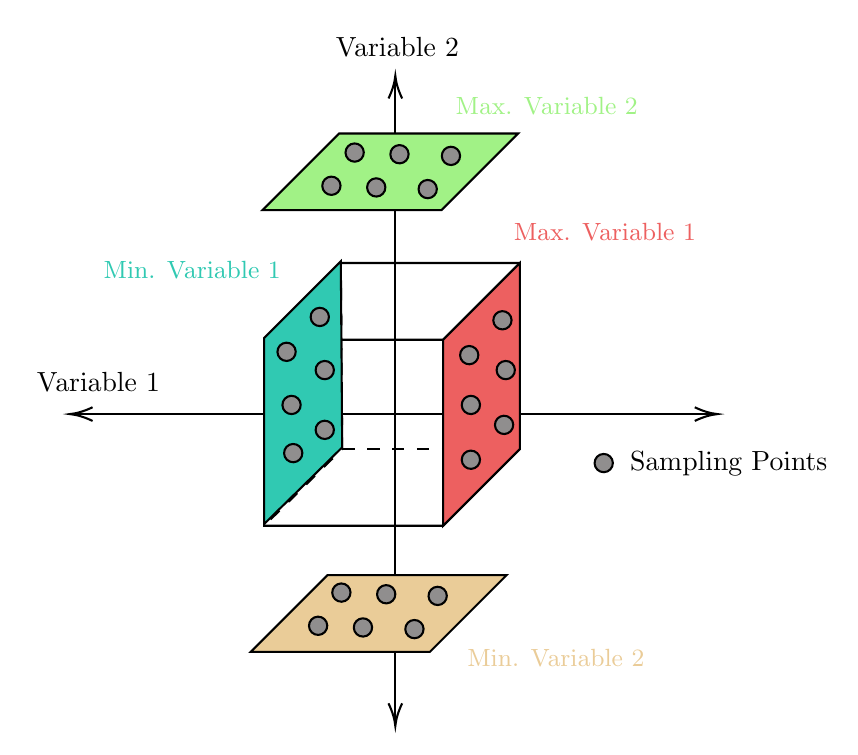
\begin{tikzpicture}[x=0.75pt,y=0.75pt,yscale=-1,xscale=1]
%uncomment if require: \path (0,426); %set diagram left start at 0, and has height of 426

%Shape: Cube [id:dp41916472639407576] 
\draw   (188.8,213.17) -- (225.77,176.2) -- (312.03,176.2) -- (312.03,265.83) -- (275.06,302.8) -- (188.8,302.8) -- cycle ; \draw   (312.03,176.2) -- (275.06,213.17) -- (188.8,213.17) ; \draw   (275.06,213.17) -- (275.06,302.8) ;
%Straight Lines [id:da1100678834838219] 
\draw    (254.4,249) -- (405.23,249) ;
\draw [shift={(407.23,249)}, rotate = 180] [color={rgb, 255:red, 0; green, 0; blue, 0 }  ][line width=0.75]    (10.93,-3.29) .. controls (6.95,-1.4) and (3.31,-0.3) .. (0,0) .. controls (3.31,0.3) and (6.95,1.4) .. (10.93,3.29)   ;
%Straight Lines [id:da8209310669516441] 
\draw    (254.4,249) -- (97.23,249) ;
\draw [shift={(95.23,249)}, rotate = 360] [color={rgb, 255:red, 0; green, 0; blue, 0 }  ][line width=0.75]    (10.93,-3.29) .. controls (6.95,-1.4) and (3.31,-0.3) .. (0,0) .. controls (3.31,0.3) and (6.95,1.4) .. (10.93,3.29)   ;
%Shape: Polygon [id:ds315102272045769] 
\draw  [dash pattern={on 4.5pt off 4.5pt}] (225.77,176.2) -- (226.43,265.83) -- (188.8,302.8) -- (188.8,213.17) -- cycle ;
%Straight Lines [id:da6924249131024756] 
\draw  [dash pattern={on 4.5pt off 4.5pt}]  (226.43,265.83) -- (312.03,265.83) ;
%Shape: Polygon [id:ds26648827466781355] 
\draw  [fill={rgb, 255:red, 237; green, 96; blue, 96 }  ,fill opacity=1 ] (312.03,176.2) -- (312.03,265.83) -- (275.06,302.8) -- (275.06,213.17) -- cycle ;
%Shape: Polygon [id:ds5376783951801227] 
\draw  [fill={rgb, 255:red, 48; green, 201; blue, 178 }  ,fill opacity=1 ] (225.77,175.4) -- (226.43,265.03) -- (188.8,302) -- (188.8,212.37) -- cycle ;
%Shape: Circle [id:dp6613928021845482] 
\draw  [fill={rgb, 255:red, 144; green, 142; blue, 142 }  ,fill opacity=1 ] (211.23,202.31) .. controls (211.16,199.88) and (213.08,197.85) .. (215.51,197.79) .. controls (217.95,197.72) and (219.97,199.64) .. (220.04,202.07) .. controls (220.1,204.51) and (218.19,206.53) .. (215.75,206.6) .. controls (213.32,206.66) and (211.29,204.75) .. (211.23,202.31) -- cycle ;
%Shape: Circle [id:dp10792302470599302] 
\draw  [fill={rgb, 255:red, 144; green, 142; blue, 142 }  ,fill opacity=1 ] (195.23,219.11) .. controls (195.16,216.68) and (197.08,214.65) .. (199.51,214.59) .. controls (201.95,214.52) and (203.97,216.44) .. (204.04,218.87) .. controls (204.1,221.31) and (202.19,223.33) .. (199.75,223.4) .. controls (197.32,223.46) and (195.29,221.55) .. (195.23,219.11) -- cycle ;
%Shape: Circle [id:dp764393572474829] 
\draw  [fill={rgb, 255:red, 144; green, 142; blue, 142 }  ,fill opacity=1 ] (213.63,227.91) .. controls (213.56,225.48) and (215.48,223.45) .. (217.91,223.39) .. controls (220.35,223.32) and (222.37,225.24) .. (222.44,227.67) .. controls (222.5,230.11) and (220.59,232.13) .. (218.15,232.2) .. controls (215.72,232.26) and (213.69,230.35) .. (213.63,227.91) -- cycle ;
%Shape: Circle [id:dp2635654509882438] 
\draw  [fill={rgb, 255:red, 144; green, 142; blue, 142 }  ,fill opacity=1 ] (197.63,244.71) .. controls (197.56,242.28) and (199.48,240.25) .. (201.91,240.19) .. controls (204.35,240.12) and (206.37,242.04) .. (206.44,244.47) .. controls (206.5,246.91) and (204.59,248.93) .. (202.15,249) .. controls (199.72,249.06) and (197.69,247.15) .. (197.63,244.71) -- cycle ;
%Shape: Circle [id:dp720401298117804] 
\draw  [fill={rgb, 255:red, 144; green, 142; blue, 142 }  ,fill opacity=1 ] (213.63,256.71) .. controls (213.56,254.28) and (215.48,252.25) .. (217.91,252.19) .. controls (220.35,252.12) and (222.37,254.04) .. (222.44,256.47) .. controls (222.5,258.91) and (220.59,260.93) .. (218.15,261) .. controls (215.72,261.06) and (213.69,259.15) .. (213.63,256.71) -- cycle ;
%Shape: Circle [id:dp3334941876745968] 
\draw  [fill={rgb, 255:red, 144; green, 142; blue, 142 }  ,fill opacity=1 ] (198.43,267.91) .. controls (198.36,265.48) and (200.28,263.45) .. (202.71,263.39) .. controls (205.15,263.32) and (207.17,265.24) .. (207.24,267.67) .. controls (207.3,270.11) and (205.39,272.13) .. (202.95,272.2) .. controls (200.52,272.26) and (198.49,270.35) .. (198.43,267.91) -- cycle ;
%Shape: Circle [id:dp9121056350905267] 
\draw  [fill={rgb, 255:red, 144; green, 142; blue, 142 }  ,fill opacity=1 ] (299.23,203.91) .. controls (299.16,201.48) and (301.08,199.45) .. (303.51,199.39) .. controls (305.95,199.32) and (307.97,201.24) .. (308.04,203.67) .. controls (308.1,206.11) and (306.19,208.13) .. (303.75,208.2) .. controls (301.32,208.26) and (299.29,206.35) .. (299.23,203.91) -- cycle ;
%Shape: Circle [id:dp461002915724564] 
\draw  [fill={rgb, 255:red, 144; green, 142; blue, 142 }  ,fill opacity=1 ] (283.23,220.71) .. controls (283.16,218.28) and (285.08,216.25) .. (287.51,216.19) .. controls (289.95,216.12) and (291.97,218.04) .. (292.04,220.47) .. controls (292.1,222.91) and (290.19,224.93) .. (287.75,225) .. controls (285.32,225.06) and (283.29,223.15) .. (283.23,220.71) -- cycle ;
%Shape: Circle [id:dp715936866594871] 
\draw  [fill={rgb, 255:red, 144; green, 142; blue, 142 }  ,fill opacity=1 ] (300.83,227.91) .. controls (300.76,225.48) and (302.68,223.45) .. (305.11,223.39) .. controls (307.55,223.32) and (309.57,225.24) .. (309.64,227.67) .. controls (309.7,230.11) and (307.79,232.13) .. (305.35,232.2) .. controls (302.92,232.26) and (300.89,230.35) .. (300.83,227.91) -- cycle ;
%Shape: Circle [id:dp5335650842060755] 
\draw  [fill={rgb, 255:red, 144; green, 142; blue, 142 }  ,fill opacity=1 ] (284.03,244.71) .. controls (283.96,242.28) and (285.88,240.25) .. (288.31,240.19) .. controls (290.75,240.12) and (292.77,242.04) .. (292.84,244.47) .. controls (292.9,246.91) and (290.99,248.93) .. (288.55,249) .. controls (286.12,249.06) and (284.09,247.15) .. (284.03,244.71) -- cycle ;
%Shape: Circle [id:dp6761023350021587] 
\draw  [fill={rgb, 255:red, 144; green, 142; blue, 142 }  ,fill opacity=1 ] (300.03,254.31) .. controls (299.96,251.88) and (301.88,249.85) .. (304.31,249.79) .. controls (306.75,249.72) and (308.77,251.64) .. (308.84,254.07) .. controls (308.9,256.51) and (306.99,258.53) .. (304.55,258.6) .. controls (302.12,258.66) and (300.09,256.75) .. (300.03,254.31) -- cycle ;
%Shape: Circle [id:dp7779527390505632] 
\draw  [fill={rgb, 255:red, 144; green, 142; blue, 142 }  ,fill opacity=1 ] (284.03,271.11) .. controls (283.96,268.68) and (285.88,266.65) .. (288.31,266.59) .. controls (290.75,266.52) and (292.77,268.44) .. (292.84,270.87) .. controls (292.9,273.31) and (290.99,275.33) .. (288.55,275.4) .. controls (286.12,275.46) and (284.09,273.55) .. (284.03,271.11) -- cycle ;
%Shape: Circle [id:dp39193327346815965] 
\draw  [fill={rgb, 255:red, 144; green, 142; blue, 142 }  ,fill opacity=1 ] (348.03,272.71) .. controls (347.96,270.28) and (349.88,268.25) .. (352.31,268.19) .. controls (354.75,268.12) and (356.77,270.04) .. (356.84,272.47) .. controls (356.9,274.91) and (354.99,276.93) .. (352.55,277) .. controls (350.12,277.06) and (348.09,275.15) .. (348.03,272.71) -- cycle ;
%Straight Lines [id:da4370737882051544] 
\draw    (252.03,397.29) -- (252.03,88) ;
\draw [shift={(252.03,86)}, rotate = 90] [color={rgb, 255:red, 0; green, 0; blue, 0 }  ][line width=0.75]    (10.93,-3.29) .. controls (6.95,-1.4) and (3.31,-0.3) .. (0,0) .. controls (3.31,0.3) and (6.95,1.4) .. (10.93,3.29)   ;
\draw [shift={(252.03,399.29)}, rotate = 270] [color={rgb, 255:red, 0; green, 0; blue, 0 }  ][line width=0.75]    (10.93,-3.29) .. controls (6.95,-1.4) and (3.31,-0.3) .. (0,0) .. controls (3.31,0.3) and (6.95,1.4) .. (10.93,3.29)   ;
%Shape: Polygon [id:ds027192625551482386] 
\draw  [fill={rgb, 255:red, 161; green, 242; blue, 134 }  ,fill opacity=1 ] (311.23,113.8) -- (274.26,150.77) -- (188,150.77) -- (224.97,113.8) -- cycle ;
%Shape: Polygon [id:ds7003641159858384] 
\draw  [fill={rgb, 255:red, 234; green, 204; blue, 152 }  ,fill opacity=1 ] (305.63,326.6) -- (268.66,363.57) -- (182.4,363.57) -- (219.37,326.6) -- cycle ;
%Shape: Circle [id:dp7862884715493691] 
\draw  [fill={rgb, 255:red, 144; green, 142; blue, 142 }  ,fill opacity=1 ] (228.03,123.11) .. controls (227.96,120.68) and (229.88,118.65) .. (232.31,118.59) .. controls (234.75,118.52) and (236.77,120.44) .. (236.84,122.87) .. controls (236.9,125.31) and (234.99,127.33) .. (232.55,127.4) .. controls (230.12,127.46) and (228.09,125.55) .. (228.03,123.11) -- cycle ;
%Shape: Circle [id:dp9269233874737624] 
\draw  [fill={rgb, 255:red, 144; green, 142; blue, 142 }  ,fill opacity=1 ] (216.83,139.11) .. controls (216.76,136.68) and (218.68,134.65) .. (221.11,134.59) .. controls (223.55,134.52) and (225.57,136.44) .. (225.64,138.87) .. controls (225.7,141.31) and (223.79,143.33) .. (221.35,143.4) .. controls (218.92,143.46) and (216.89,141.55) .. (216.83,139.11) -- cycle ;
%Shape: Circle [id:dp9900121536496537] 
\draw  [fill={rgb, 255:red, 144; green, 142; blue, 142 }  ,fill opacity=1 ] (249.63,123.91) .. controls (249.56,121.48) and (251.48,119.45) .. (253.91,119.39) .. controls (256.35,119.32) and (258.37,121.24) .. (258.44,123.67) .. controls (258.5,126.11) and (256.59,128.13) .. (254.15,128.2) .. controls (251.72,128.26) and (249.69,126.35) .. (249.63,123.91) -- cycle ;
%Shape: Circle [id:dp0010559062693412669] 
\draw  [fill={rgb, 255:red, 144; green, 142; blue, 142 }  ,fill opacity=1 ] (238.43,139.91) .. controls (238.36,137.48) and (240.28,135.45) .. (242.71,135.39) .. controls (245.15,135.32) and (247.17,137.24) .. (247.24,139.67) .. controls (247.3,142.11) and (245.39,144.13) .. (242.95,144.2) .. controls (240.52,144.26) and (238.49,142.35) .. (238.43,139.91) -- cycle ;
%Shape: Circle [id:dp9729939432021396] 
\draw  [fill={rgb, 255:red, 144; green, 142; blue, 142 }  ,fill opacity=1 ] (274.43,124.71) .. controls (274.36,122.28) and (276.28,120.25) .. (278.71,120.19) .. controls (281.15,120.12) and (283.17,122.04) .. (283.24,124.47) .. controls (283.3,126.91) and (281.39,128.93) .. (278.95,129) .. controls (276.52,129.06) and (274.49,127.15) .. (274.43,124.71) -- cycle ;
%Shape: Circle [id:dp5583563494601032] 
\draw  [fill={rgb, 255:red, 144; green, 142; blue, 142 }  ,fill opacity=1 ] (263.23,140.71) .. controls (263.16,138.28) and (265.08,136.25) .. (267.51,136.19) .. controls (269.95,136.12) and (271.97,138.04) .. (272.04,140.47) .. controls (272.1,142.91) and (270.19,144.93) .. (267.75,145) .. controls (265.32,145.06) and (263.29,143.15) .. (263.23,140.71) -- cycle ;
%Shape: Circle [id:dp2803403187081903] 
\draw  [fill={rgb, 255:red, 144; green, 142; blue, 142 }  ,fill opacity=1 ] (221.63,335.11) .. controls (221.56,332.68) and (223.48,330.65) .. (225.91,330.59) .. controls (228.35,330.52) and (230.37,332.44) .. (230.44,334.87) .. controls (230.5,337.31) and (228.59,339.33) .. (226.15,339.4) .. controls (223.72,339.46) and (221.69,337.55) .. (221.63,335.11) -- cycle ;
%Shape: Circle [id:dp08580816994108764] 
\draw  [fill={rgb, 255:red, 144; green, 142; blue, 142 }  ,fill opacity=1 ] (210.43,351.11) .. controls (210.36,348.68) and (212.28,346.65) .. (214.71,346.59) .. controls (217.15,346.52) and (219.17,348.44) .. (219.24,350.87) .. controls (219.3,353.31) and (217.39,355.33) .. (214.95,355.4) .. controls (212.52,355.46) and (210.49,353.55) .. (210.43,351.11) -- cycle ;
%Shape: Circle [id:dp8920356550311489] 
\draw  [fill={rgb, 255:red, 144; green, 142; blue, 142 }  ,fill opacity=1 ] (243.23,335.91) .. controls (243.16,333.48) and (245.08,331.45) .. (247.51,331.39) .. controls (249.95,331.32) and (251.97,333.24) .. (252.04,335.67) .. controls (252.1,338.11) and (250.19,340.13) .. (247.75,340.2) .. controls (245.32,340.26) and (243.29,338.35) .. (243.23,335.91) -- cycle ;
%Shape: Circle [id:dp9149486091931166] 
\draw  [fill={rgb, 255:red, 144; green, 142; blue, 142 }  ,fill opacity=1 ] (232.03,351.91) .. controls (231.96,349.48) and (233.88,347.45) .. (236.31,347.39) .. controls (238.75,347.32) and (240.77,349.24) .. (240.84,351.67) .. controls (240.9,354.11) and (238.99,356.13) .. (236.55,356.2) .. controls (234.12,356.26) and (232.09,354.35) .. (232.03,351.91) -- cycle ;
%Shape: Circle [id:dp453151861693878] 
\draw  [fill={rgb, 255:red, 144; green, 142; blue, 142 }  ,fill opacity=1 ] (268.03,336.71) .. controls (267.96,334.28) and (269.88,332.25) .. (272.31,332.19) .. controls (274.75,332.12) and (276.77,334.04) .. (276.84,336.47) .. controls (276.9,338.91) and (274.99,340.93) .. (272.55,341) .. controls (270.12,341.06) and (268.09,339.15) .. (268.03,336.71) -- cycle ;
%Shape: Circle [id:dp2654623156037197] 
\draw  [fill={rgb, 255:red, 144; green, 142; blue, 142 }  ,fill opacity=1 ] (256.83,352.71) .. controls (256.76,350.28) and (258.68,348.25) .. (261.11,348.19) .. controls (263.55,348.12) and (265.57,350.04) .. (265.64,352.47) .. controls (265.7,354.91) and (263.79,356.93) .. (261.35,357) .. controls (258.92,357.06) and (256.89,355.15) .. (256.83,352.71) -- cycle ;

% Text Node
\draw (108.99,233.5) node   [align=left] {Variable 1};
% Text Node
\draw (279.6,94.6) node [anchor=north west][inner sep=0.75pt]  [font=\small,color={rgb, 255:red, 161; green, 242; blue, 134 }  ,opacity=1 ] [align=left] {Max. Variable 2};
% Text Node
\draw (307.6,155.4) node [anchor=north west][inner sep=0.75pt]  [font=\small,color={rgb, 255:red, 237; green, 96; blue, 96 }  ,opacity=1 ] [align=left] {Max. Variable 1};
% Text Node
\draw (363.6,265.4) node [anchor=north west][inner sep=0.75pt]   [align=left] {Sampling Points};
% Text Node
\draw (252.99,71.9) node   [align=left] {Variable 2};
% Text Node
\draw (110,173.8) node [anchor=north west][inner sep=0.75pt]  [font=\small,color={rgb, 255:red, 48; green, 201; blue, 178 }  ,opacity=1 ] [align=left] {Min. Variable 1};
% Text Node
\draw (285.2,361) node [anchor=north west][inner sep=0.75pt]  [font=\small,color={rgb, 255:red, 234; green, 204; blue, 152 }  ,opacity=1 ] [align=left] {Min. Variable 2};

\end{tikzpicture}
\caption{Data sampling strategy following a Latin Hypercube approach. The minimum and maximum value for each variable is fixed and $n$ data points are chosen, which creates $n_{variables}\times n_{points}\times 2$ experiments}
\label{fig: hypercube}
\end{figure}



By using $n$ number of design variables, this concept expands to an $n$-dimensional hypercube. This allows us to explore a broader design space, making sure that every point data is meaningful, as it represents a unique combination of potentials. In this paper, we utilized 25 sampling points, ie: there are 25 data points in each of the faces of the cube, creating $4\times 25 \times 2=200$ different combinations of potentials.

These potentials will be used as an input for the finite element analysis, in the form of a 4-element vector (the potential at each electrode). Moreover, since 200 experiments will likely be unsufficient to capture the complex phenomena behind this dielectric elastomer using a machine learning model, we will enrich this data further. To do so, we will take advantage of the load-stepping scheme implemented in the finite element analysis. Load-stepping allows for an easier convergence of the Newton-Raphson algorithm. By applying a fraction of the total load at the beginning of the analysis, solving the Newton-Raphson and then increasing the load, we can better capture non-linearities, increasing convergence. 

Utilizing these intermediate data, we can extend the initial 200 finite element samples, to over 20000, accounting for possible cutbacks and bisections during the load-stepping, which will further increase the data available. For each load (combination of potentials), we also needed to store the displacement output. For ease of access and convenience, we projected the displacement of all the nodes to one of the top surfaces of the dielectric elastomer, which contains 133 nodes. Hence, for each 4-element vector load, we will have a corresponding 399-element vector of displacement (coordinates 1, 2 and 3 of each of the 133 points). These will be our training and test samples.


\subsubsection{Training strategy}

The goal now is to train a neural network to accurately predict the displacement of the dielectric elastomer for a given input potential. Hence, the input for the neural network is a 4-element vector and the output is a 399-element vector. However, since the primary deformation mechanisms will be bending and torsion, the effect of shear deformation is negligible. This allows us to effectively remove one of the components of the displacements, namely the one that represents the movement in axial direction. As a result, the original 399-element data is reduced to 266-element data, which holds only displacements in the first and third coordinate directions. 

Using this data, we can train a neural network that predicts the displacement for a given combination of potentials. However, the proper architecture to do this prediction is unknown at this stage. There is no clear direction in which the hyperparemeters of the neural network need to be changed in order to achieve reasonable prediction capabilities. For this reason, a parametric study was carried out in which neural network calibration is done by varying different hyperparameter values. Namely: the number of nodes ($n_{nodes}$), the number of neurons ($n_{neurons}$), the number of experiments ($n_{experiments}$) and the number of layers ($n_{layers}$). To study the convergence of the machine learning model, the number of epochs was also introduced in the parametric study.



\tikzset{every picture/.style={line width=0.75pt}} %set default line width to 0.75pt        
\begin{figure}
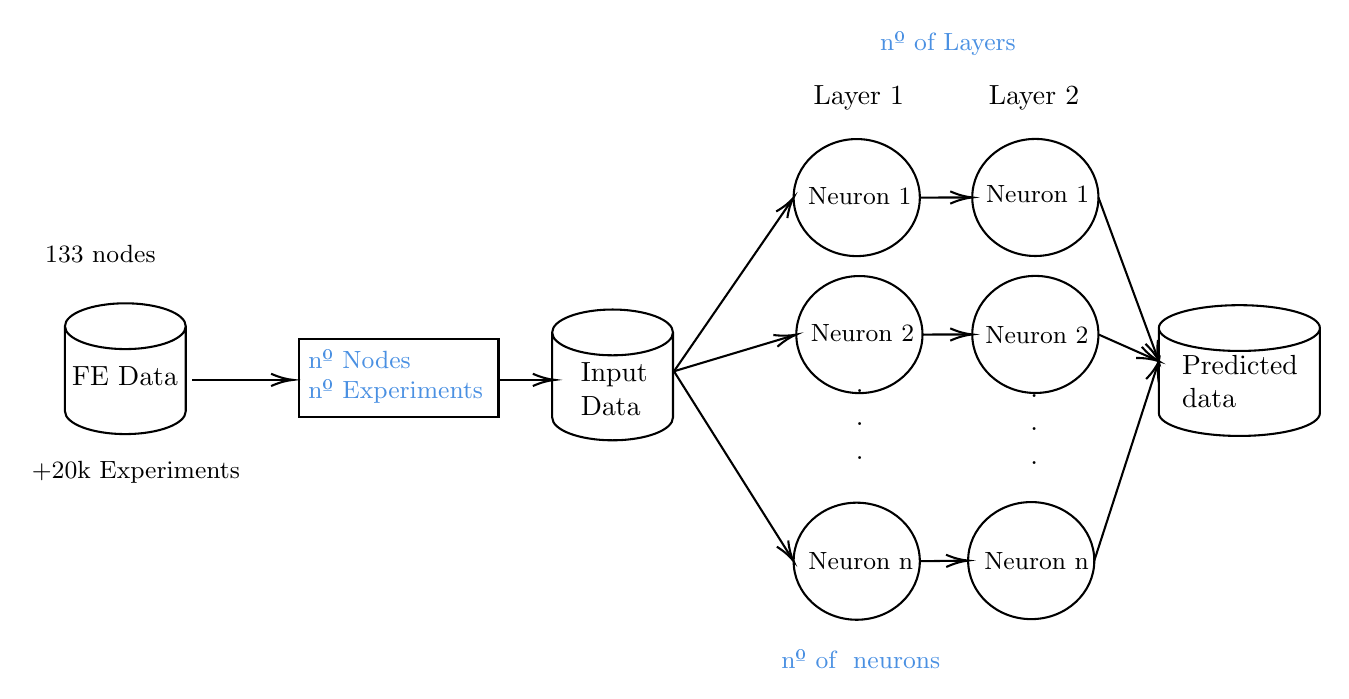
\begin{tikzpicture}[x=0.75pt,y=0.75pt,yscale=-0.9,xscale=0.97]
%uncomment if require: \path (0,444); %set diagram left start at 0, and has height of 444

%Shape: Circle [id:dp7149132561338333] 
\draw   (388.61,102.4) .. controls (388.61,85.1) and (402.64,71.07) .. (419.94,71.07) .. controls (437.25,71.07) and (451.28,85.1) .. (451.28,102.4) .. controls (451.28,119.7) and (437.25,133.73) .. (419.94,133.73) .. controls (402.64,133.73) and (388.61,119.7) .. (388.61,102.4) -- cycle ;
%Shape: Circle [id:dp013523830492098043] 
\draw   (389.94,175.73) .. controls (389.94,158.43) and (403.97,144.4) .. (421.28,144.4) .. controls (438.58,144.4) and (452.61,158.43) .. (452.61,175.73) .. controls (452.61,193.04) and (438.58,207.07) .. (421.28,207.07) .. controls (403.97,207.07) and (389.94,193.04) .. (389.94,175.73) -- cycle ;
%Shape: Circle [id:dp6349374096098536] 
\draw   (388.61,297.07) .. controls (388.61,279.76) and (402.64,265.73) .. (419.94,265.73) .. controls (437.25,265.73) and (451.28,279.76) .. (451.28,297.07) .. controls (451.28,314.37) and (437.25,328.4) .. (419.94,328.4) .. controls (402.64,328.4) and (388.61,314.37) .. (388.61,297.07) -- cycle ;
%Flowchart: Magnetic Disk [id:dp2804160649676165] 
\draw   (86.67,171.25) -- (86.67,216.75) .. controls (86.67,223.52) and (73.24,229) .. (56.67,229) .. controls (40.1,229) and (26.67,223.52) .. (26.67,216.75) -- (26.67,171.25)(86.67,171.25) .. controls (86.67,178.02) and (73.24,183.5) .. (56.67,183.5) .. controls (40.1,183.5) and (26.67,178.02) .. (26.67,171.25) .. controls (26.67,164.48) and (40.1,159) .. (56.67,159) .. controls (73.24,159) and (86.67,164.48) .. (86.67,171.25) -- cycle ;
%Flowchart: Magnetic Disk [id:dp6592793249759878] 
\draw   (328.67,174.58) -- (328.67,220.08) .. controls (328.67,226.85) and (315.24,232.33) .. (298.67,232.33) .. controls (282.1,232.33) and (268.67,226.85) .. (268.67,220.08) -- (268.67,174.58)(328.67,174.58) .. controls (328.67,181.35) and (315.24,186.83) .. (298.67,186.83) .. controls (282.1,186.83) and (268.67,181.35) .. (268.67,174.58) .. controls (268.67,167.82) and (282.1,162.33) .. (298.67,162.33) .. controls (315.24,162.33) and (328.67,167.82) .. (328.67,174.58) -- cycle ;
%Straight Lines [id:da35532704073807175] 
\draw    (387.53,104.09) -- (329.17,195.39) ;
\draw [shift={(388.61,102.4)}, rotate = 122.59] [color={rgb, 255:red, 0; green, 0; blue, 0 }  ][line width=0.75]    (10.93,-3.29) .. controls (6.95,-1.4) and (3.31,-0.3) .. (0,0) .. controls (3.31,0.3) and (6.95,1.4) .. (10.93,3.29)   ;
%Straight Lines [id:da4511032574004499] 
\draw    (388.04,176.35) -- (329.17,195.39) ;
\draw [shift={(389.94,175.73)}, rotate = 162.08] [color={rgb, 255:red, 0; green, 0; blue, 0 }  ][line width=0.75]    (10.93,-3.29) .. controls (6.95,-1.4) and (3.31,-0.3) .. (0,0) .. controls (3.31,0.3) and (6.95,1.4) .. (10.93,3.29)   ;
%Straight Lines [id:da19079915385094404] 
\draw    (387.6,295.34) -- (329.17,195.39) ;
\draw [shift={(388.61,297.07)}, rotate = 239.69] [color={rgb, 255:red, 0; green, 0; blue, 0 }  ][line width=0.75]    (10.93,-3.29) .. controls (6.95,-1.4) and (3.31,-0.3) .. (0,0) .. controls (3.31,0.3) and (6.95,1.4) .. (10.93,3.29)   ;
%Shape: Circle [id:dp7482248959951554] 
\draw   (477.33,102.33) .. controls (477.33,85.03) and (491.36,71) .. (508.67,71) .. controls (525.97,71) and (540,85.03) .. (540,102.33) .. controls (540,119.64) and (525.97,133.67) .. (508.67,133.67) .. controls (491.36,133.67) and (477.33,119.64) .. (477.33,102.33) -- cycle ;
%Shape: Circle [id:dp5965819972858774] 
\draw   (477.33,175.67) .. controls (477.33,158.36) and (491.36,144.33) .. (508.67,144.33) .. controls (525.97,144.33) and (540,158.36) .. (540,175.67) .. controls (540,192.97) and (525.97,207) .. (508.67,207) .. controls (491.36,207) and (477.33,192.97) .. (477.33,175.67) -- cycle ;
%Shape: Circle [id:dp5648862567333319] 
\draw   (475.28,296.73) .. controls (475.28,279.43) and (489.31,265.4) .. (506.61,265.4) .. controls (523.92,265.4) and (537.94,279.43) .. (537.94,296.73) .. controls (537.94,314.04) and (523.92,328.07) .. (506.61,328.07) .. controls (489.31,328.07) and (475.28,314.04) .. (475.28,296.73) -- cycle ;
%Straight Lines [id:da8586261828242774] 
\draw    (451.28,102.4) -- (475.33,102.34) ;
\draw [shift={(477.33,102.33)}, rotate = 179.85] [color={rgb, 255:red, 0; green, 0; blue, 0 }  ][line width=0.75]    (10.93,-3.29) .. controls (6.95,-1.4) and (3.31,-0.3) .. (0,0) .. controls (3.31,0.3) and (6.95,1.4) .. (10.93,3.29)   ;
%Straight Lines [id:da7717426599628258] 
\draw    (452.61,175.73) -- (475.33,175.67) ;
\draw [shift={(477.33,175.67)}, rotate = 179.85] [color={rgb, 255:red, 0; green, 0; blue, 0 }  ][line width=0.75]    (10.93,-3.29) .. controls (6.95,-1.4) and (3.31,-0.3) .. (0,0) .. controls (3.31,0.3) and (6.95,1.4) .. (10.93,3.29)   ;
%Straight Lines [id:da3046916071479544] 
\draw    (451.28,297.07) -- (473.28,296.76) ;
\draw [shift={(475.28,296.73)}, rotate = 179.2] [color={rgb, 255:red, 0; green, 0; blue, 0 }  ][line width=0.75]    (10.93,-3.29) .. controls (6.95,-1.4) and (3.31,-0.3) .. (0,0) .. controls (3.31,0.3) and (6.95,1.4) .. (10.93,3.29)   ;
%Straight Lines [id:da6640975488428904] 
\draw    (90,200) -- (138,200) ;
\draw [shift={(140,200)}, rotate = 180] [color={rgb, 255:red, 0; green, 0; blue, 0 }  ][line width=0.75]    (10.93,-3.29) .. controls (6.95,-1.4) and (3.31,-0.3) .. (0,0) .. controls (3.31,0.3) and (6.95,1.4) .. (10.93,3.29)   ;
%Straight Lines [id:da6892392743456469] 
\draw    (243,200) -- (268,200) ;
\draw [shift={(270,200)}, rotate = 180] [color={rgb, 255:red, 0; green, 0; blue, 0 }  ][line width=0.75]    (10.93,-3.29) .. controls (6.95,-1.4) and (3.31,-0.3) .. (0,0) .. controls (3.31,0.3) and (6.95,1.4) .. (10.93,3.29)   ;
%Flowchart: Magnetic Disk [id:dp35749579079078997] 
\draw   (650,172.25) -- (650,217.75) .. controls (650,224.52) and (632.09,230) .. (610,230) .. controls (587.91,230) and (570,224.52) .. (570,217.75) -- (570,172.25)(650,172.25) .. controls (650,179.02) and (632.09,184.5) .. (610,184.5) .. controls (587.91,184.5) and (570,179.02) .. (570,172.25) .. controls (570,165.48) and (587.91,160) .. (610,160) .. controls (632.09,160) and (650,165.48) .. (650,172.25) -- cycle ;
%Straight Lines [id:da5896782313243266] 
\draw    (540,102.33) -- (569.35,188.11) ;
\draw [shift={(570,190)}, rotate = 251.11] [color={rgb, 255:red, 0; green, 0; blue, 0 }  ][line width=0.75]    (10.93,-3.29) .. controls (6.95,-1.4) and (3.31,-0.3) .. (0,0) .. controls (3.31,0.3) and (6.95,1.4) .. (10.93,3.29)   ;
%Straight Lines [id:da28421655439140037] 
\draw    (540,175.67) -- (568.2,189.14) ;
\draw [shift={(570,190)}, rotate = 205.54] [color={rgb, 255:red, 0; green, 0; blue, 0 }  ][line width=0.75]    (10.93,-3.29) .. controls (6.95,-1.4) and (3.31,-0.3) .. (0,0) .. controls (3.31,0.3) and (6.95,1.4) .. (10.93,3.29)   ;
%Straight Lines [id:da846956632663103] 
\draw    (537.94,296.73) -- (569.42,191.92) ;
\draw [shift={(570,190)}, rotate = 106.72] [color={rgb, 255:red, 0; green, 0; blue, 0 }  ][line width=0.75]    (10.93,-3.29) .. controls (6.95,-1.4) and (3.31,-0.3) .. (0,0) .. controls (3.31,0.3) and (6.95,1.4) .. (10.93,3.29)   ;

% Text Node
\draw (422.79,175.12) node  [font=\small] [align=left] {Neuron 2};
% Text Node
\draw (421.94,296.94) node  [font=\small] [align=left] {Neuron n};
% Text Node
\draw (418,203.67) node [anchor=north west][inner sep=0.75pt]   [align=left] {.\\.\\.};
% Text Node
\draw (28.67,191.33) node [anchor=north west][inner sep=0.75pt]   [align=left] {FE Data};
% Text Node
\draw    (143,178) -- (242,178) -- (242,220) -- (143,220) -- cycle  ;
\draw (146,182) node [anchor=north west][inner sep=0.75pt]  [font=\small,color={rgb, 255:red, 74; green, 144; blue, 226 }  ,opacity=1 ] [align=left] {nº Nodes\\nº Experiments};
% Text Node
\draw (15.33,126) node [anchor=north west][inner sep=0.75pt]  [font=\small,color={rgb, 255:red, 0; green, 0; blue, 0 }  ,opacity=1 ] [align=left] {133 nodes};
% Text Node
\draw (8.67,242) node [anchor=north west][inner sep=0.75pt]  [font=\small] [align=left] {+20k Experiments};
% Text Node
\draw (281.33,189.33) node [anchor=north west][inner sep=0.75pt]   [align=left] {Input \\Data};
% Text Node
\draw (509.46,175.78) node  [font=\small] [align=left] {Neuron 2};
% Text Node
\draw (509.28,296.94) node  [font=\small] [align=left] {Neuron n};
% Text Node
\draw (504.67,206.33) node [anchor=north west][inner sep=0.75pt]   [align=left] {.\\.\\.};
% Text Node
\draw (421.46,101.78) node  [font=\small] [align=left] {Neuron 1};
% Text Node
\draw (509.79,100.45) node  [font=\small] [align=left] {Neuron 1};
% Text Node
\draw (397,41) node [anchor=north west][inner sep=0.75pt]   [align=left] {Layer 1};
% Text Node
\draw (484,41) node [anchor=north west][inner sep=0.75pt]   [align=left] {Layer 2};
% Text Node
\draw (580,185) node [anchor=north west][inner sep=0.75pt]   [align=left] {Predicted \\data\\};
% Text Node
\draw (430,12) node [anchor=north west][inner sep=0.75pt]  [font=\small,color={rgb, 255:red, 74; green, 144; blue, 226 }  ,opacity=1 ] [align=left] {nº of Layers};
% Text Node
\draw (381,343) node [anchor=north west][inner sep=0.75pt]  [font=\small,color={rgb, 255:red, 74; green, 144; blue, 226 }  ,opacity=1 ] [align=left] {nº of \ neurons};


\end{tikzpicture}
\caption{Training process schematic. The number of variables modified during the parametric study can be seen in blue.}
\end{figure}
Alongside architecture-specific parameters, like the number of neurons, the number of layers and the number of epochs, we also studied the effect of the number of nodes and experiments. From the available 266 nodes, we took only a subset of them and used them to train the neural network, leaving the remaining nodes as test data to compare against. The same concept is used by selecting only a subset of experiments out of the ones available. The purpose of this subset selection is calibrating a neural network that is able to predict the complete response, reducing the computational expense without losing accuracy by reducing the number of nodes and experiments used. 

For each of the hyperparameters specified, the values studied were the following:

\begin{table}[!hb]
  \centering
\begin{tabular}{l|cccc}
\textbf{Parameters} & \multicolumn{3}{c}{\textbf{Value}} \\ \hline
Layers              & 4      & 8       & 10            \\
Neurons             & 10     & 20      & 40           \\
Experiments         & 2077    & 7000    & 10000      \\
Nodes               & 50     & 10      & 200           \\
Epochs              &  \multicolumn{3}{c}{1e4}        
\end{tabular}
  \caption{Values used in the parametric study during the training phase. Every combination of these parameters was analysed and parsed to obtain the best performing architecture.}
\end{table}

\subsubsection{Results}


Every possible combination of these parameters was studied, totalling 81 different architectures that were run and analysed. To measure the performance of these architectures, the R2 measurement (\ref{eq:R2_measurement}), was used. This metric allows us to compare the displacements predicted by the neural network against the test data (the remaining data that was not taken into the training process). To provide a clearer outlook on the results of the parametric hyperparameter study, we compiled the output of R2 measurements on every combination of 50 and 200 nodes using 2077 and 10000 experiments. These results can be visualized in Table \ref{tab: R2_measurement}. By analyzing only a subset of 36 architectures out of the total 81, we can establish different relationships between the hyperparameters used in the parametric study, namely: the number of nodes ($n_{nodes}$), the number of neurons ($n_{neurons}$), the number of experiments ($n_{experiments}$) and the number of layers ($n_{layers}$), and how they impact the quality of the predicted output. 


\begin{itemize}
  \item $n_{neurons}$: The number of neurons per layer is directly related to the complexity that the neural network can handle. More neurons per layer means more complex relationships that can be established between each neuron, allowing for deeper understanding of the problem. However, a high number of neurons can overfit the problem, missing generalization and causing low accuracy. In order to control the overfitting behaviour, the training process computes the R2 of the training data, as well as the test data, meaning that even if there is a high R2 at the training points (good training strategy), we will not miss generalization and the overall context of the problem. Hence, the higher the number of neurons, the better predictions we will obtain. 
  \item  $n_{layers}$: The number of layers is often referred to as the \textit{depth} of the neural network. The deeper the network, the better its ability to understand complex patterns among the data. In our example, the depth of the network is crucial to capture the nonlinear phenomena that characterises the electromechanic problem of a dielectric elastomer. Hence, more layers will allow us to better depict the deformantion accross multiple potential combinations.
  \item $n_{nodes}$: Out of the total number of nodes available in the top surface of the elastomer, we are selecting only a subset, referred to as $\alpha_n$, where $n$ is the number of nodes in the subset. This reduced dataset of nodal displacement data is related to the amount of information that will be provided to the neural network. By using the full nodal displacement data available, we would be able to predict the displacement at each node accurately, but at a cost of computational efficiency and generalization. Hence, more nodes will mean a broader description of the complete deformation mode of the elastomer. However, this is not related to the accuracy of the neural network, but to how well the network is able to predict the overall physical behaviour. Subsequently, more nodes does not mean higher accuracy.
  \item  $n_{experiments}$: The number of experiments refers to the amount of combination of potentials that will be fed to the neural network. More experiments used in the training phase will allow the network to better predict the complete test dataset of potential combinations used. Nonetheless, an increase in the amount of experiments used in the training phase will result in higher computational cost. 
\end{itemize}

We have summarized the effect of the 4 parameters in table \ref{table:summary_NN_params}

\begin{figure}
\centering

\begin{tabular}{|c|c|}
    \hline
    \textbf{Parameter} & \textbf{Effect on \( R^2 \)} \\ 
    \hline
    Number of Neurons & \textbf{↑ Improves}, but \textbf{↓ overfits if too high} \\ 
    \hline
    Number of Layers & \textbf{↑ Improves}, but \textbf{↓ may plateau} \\ 
    \hline
    Experiments (Data) & \textbf{↑ Always improves} (more data = better generalization) \\ 
    \hline
    Nodes Used & \textbf{↑ Helps} with generalization, but \textbf{not} related to the accuracy  \\ 
    \hline

\end{tabular}
  
  \caption{Summary table on the effect of the number of neurons, nodes, layers and experiments on the accuracy of the neural network, measured via the R2 value}
  \label{table:summary_NN_params}
\end{figure}


The same qualitative influence of the parameters on the R2 value can be visualize by a spider plot \ref{fig:spiderweb}, where the inner polygon represents the influence of each parameter on the accuracy of the neural network. 

\newcommand{\D}{4} % number of dimensions (config option)
\newcommand{\U}{4} % number of scale units (config option)

\newdimen\R % maximal diagram radius (config option)
\R=3.5cm 
\newdimen\L % radius to put dimension labels (config option)
\L=4cm

\newcommand{\A}{360/\D} % calculated angle between dimension axes  

\begin{figure}[htbp]
 \centering

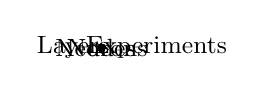
\begin{tikzpicture}[scale=1]
  \path (0:0cm) coordinate (O); % define coordinate for origin

  % draw the spiderweb (only 1 inner polygon)
  \foreach \X in {1,...,\D}{
    \draw (\X*\A:0) -- (\X*\A:\R);
  }

  % Define coordinates for the data points aligned with the axis vertices
  \path (1*\A:3.1*\R/\U) coordinate (D1);  % Neurons (similar to layers)
  \path (2*\A:3.5*\R/\U) coordinate (D2);  % Layers (mid influence)
  \path (3*\A:1*\R/\U) coordinate (D3);  % Nodes (almost 0 influence)
  \path (4*\A:3.9*\R/\U) coordinate (D4);  % Experiments (most influence)

  % Draw the inner polygon and fill it with red color for clarity
  \fill[red,opacity=0.3] (D1) -- (D2) -- (D3) -- (D4) -- cycle; % Shaded inner polygon

  % Draw the border of the inner polygon (thicker line)
  \draw [color=red,line width=2pt,opacity=0.7]
    (D1) --
    (D2) --
    (D3) --
    (D4) -- cycle; % Example polygon

  % define labels for each dimension axis (names config option)
  \path (1*\A:\L) node (L1) {\small Neurons};
  \path (2*\A:\L+0.36cm) node (L2) {\small Layers};
  \path (3*\A:\L) node (L3) {\small Nodes};
  \path (4*\A:\L+0.7cm) node (L4) {\small Experiments}; % Adjusted label position

  % draw scale lines for 4 scale units
  \foreach \Y in {1,2,3,4} {
    \foreach \X in {1,...,\D}{
      \path (\X*\A:\Y*\R/\U) coordinate (D\X-\Y);
      \fill (D\X-\Y) circle (1.5pt); % Increased size of node points
    }
    \draw [opacity=0.3] (0:\Y*\R/\U) \foreach \X in {1,...,\D}{
        -- (\X*\A:\Y*\R/\U)
    } -- cycle;
  }

\end{tikzpicture}
  \caption{Spiderweb Diagram to show the influence of 4 parameters: the number of nodes, neurons, layers and experiments on the accuracy of the neural network. Each parameter is positioned in a different axis. The higher the influence, the more area covered by the inner polygon, colored in red. By taking a look at the spiderweb figure, we can see that the parameter with the most influence is the number of experiments, followed by the number of neurons and layers. The number of nodes does not affect accuracy (high R2 value), but generalization. }
\label{fig:spiderweb}
\end{figure}



% I will take 4 combinations of n_nodes and n_experiments



% n_nodes = 10
% n_experiments=4000
% iter = 5000

%n_nodes = 10 
% n_experiments=2000
% iter = 5000


%n_nodes = 30 
% n_experiments=4000
% iter = 5000

%n_nodes = 30 
% n_experiments=2000
% iter = 5000

% Please add the following required packages to your document preamble:
% \usepackage{multirow}
% Please add the following required packages to your document preamble:
% \usepackage{multirow}
\pagebreak
\begin{table}[!hb]
\centering
\begin{minipage}{.45\textwidth}

\begin{tabular}{lllllllcc|ccc}
\multicolumn{9}{c|}{\multirow{2}{*}{\begin{tabular}[c]{@{}c@{}}$n_{nodes}=50$\\ $n_{experiments}=2077$\end{tabular}}} & \multicolumn{3}{c}{$n_{neurons}$} \\
\multicolumn{9}{c|}{}                                                                                                 & 10        & 20        & 40        \\ \hline
        &         &         &         &         &         &         & \multirow{4}{*}{\rotatebox{90}{$n_{layers}$}}        & 4        &  0.9969        &  0.9971        &  0.9990        \\
        &         &         &         &         &         &         &                                      & 8        &  0.9960        &  0.9985       &  0.9973        \\
        &         &         &         &         &         &         &                                      & 10        &  0.9970        &  0.9985        &  0.9990        
\end{tabular}

\end{minipage}

  \vspace{1cm}
\begin{minipage}{.45\textwidth}

\begin{tabular}{lllllllcc|ccc}
\multicolumn{9}{c|}{\multirow{2}{*}{\begin{tabular}[c]{@{}c@{}}$n_{nodes}=50$\\ $n_{experiments}=10000$\end{tabular}}} & \multicolumn{3}{c}{$n_{neurons}$} \\
\multicolumn{9}{c|}{}                                                                                                 & 10        & 20        & 40        \\ \hline
        &         &         &         &         &         &         & \multirow{4}{*}{\rotatebox{90}{$n_{layers}$}}        & 4        &  0.9953        &  0.9986        &  0.9989        \\
        &         &         &         &         &         &         &                                      & 8        &  0.9968        &  0.9982       &  0.9987        \\
        &         &         &         &         &         &         &                                      & 10        &  0.9965        &  0.9983        &  0.9990        
\end{tabular}

\end{minipage}

  \vspace{1cm}
\begin{minipage}{.45\textwidth}

\begin{tabular}{lllllllcc|ccc}
\multicolumn{9}{c|}{\multirow{2}{*}{\begin{tabular}[c]{@{}c@{}}$n_{nodes}=200$\\ $n_{experiments}=2077$\end{tabular}}} & \multicolumn{3}{c}{$n_{neurons}$} \\
\multicolumn{9}{c|}{}                                                                                                 & 10        & 20        & 40        \\ \hline
        &         &         &         &         &         &         & \multirow{4}{*}{\rotatebox{90}{$n_{layers}$}}        & 4        &  0.9966        &  0.9980        &  0.9988        \\
        &         &         &         &         &         &         &                                      & 8        &  0.9962        &  0.9982       &  0.9984        \\
        &         &         &         &         &         &         &                                      & 10        &  0.9891        &  0.9978        &  0.9977        
\end{tabular}

\end{minipage}

  \vspace{1cm}
\begin{minipage}{.45\textwidth}

\begin{tabular}{lllllllcc|ccc}
\multicolumn{9}{c|}{\multirow{2}{*}{\begin{tabular}[c]{@{}c@{}}$n_{nodes}=200$\\ $n_{experiments}=10000$\end{tabular}}} & \multicolumn{3}{c}{$n_{neurons}$} \\
\multicolumn{9}{c|}{}                                                                                                 & 10        & 20        & 40        \\ \hline
        &         &         &         &         &         &         & \multirow{4}{*}{\rotatebox{90}{$n_{layers}$}}        & 4        &  0.9944        &  0.9981        &  0.9991        \\
        &         &         &         &         &         &         &                                      & 8        &  0.9958        &  0.9976       &  0.9995        \\
        &         &         &         &         &         &         &                                      & 10        &  0.9971        &  0.9977        &  0.9969        
\end{tabular}

\end{minipage}





  \caption{R2 measurement for every combination of neurons and layers for 50 and 200 nodes and 2077 and 10000 experiments.}
  \label{tab: R2_values}
\end{table}


Out of the analysed architectures in Table \ref{tab: R2_values}, the best configuration is a combination of 8 layers, 40 neurons, 10000 experiments, 200 nodes  with an R2 on the test cases of 0.9995. 

To measure the dispersion of the data generated from the Machine Learning model against the in-silico FE data, we plotted the output displacement from the FE analysis against the displacement predicted by the Machine Learning architecture. Since the displacement data is given per axis in the global coordinate system, we compared the displacement per axis; namely the first and third axis. The output of this analysis is displayed in Figure \ref{fig: R2_plot} for various architectures tested.
\pagebreak
\begin{figure}[H]
  \centering
  \subfloat[Displacement in the first axis of the coordinate system of the best performing architecture: 8 layers | 40 neurons | 10000 experiments | 200 nodes]{\includegraphics[width=0.45\linewidth]{Figures/NeuralNetworkStudy/R2_Coord1_corrected_V3_mod.jpg}} \qquad
  \subfloat[Displacement in the third axis of the coordinate system of the best performing architecture: 8 layers | 40 neurons | 10000 experiments | 200 nodes]{\includegraphics[width=0.45\linewidth]{Figures/NeuralNetworkStudy/R2_Coord3_corrected_V3_mod.jpg}}\\
  \subfloat[Displacement in the first axis of the coordinate system of the architecture: 4 layers | 10 neurons | 2077 experiments | 50 nodes]{\includegraphics[width=0.45\linewidth]{Figures/NeuralNetworkStudy/R2_Coord1_corrected_V3_L4_N10_E2077_NN50_mod.jpg}}\qquad
  \subfloat[Displacement in the third axis of the coordinate system of the architecture: 4 layers | 10 neurons | 2077 experiments | 50 nodes]{\includegraphics[width=0.45\linewidth]{Figures/NeuralNetworkStudy/R2_Coord3_corrected_V3_L4_N10_E2077_NN50_mod.jpg}}
\end{figure}
\begin{figure}[H]
  \centering
  \subfloat[Displacement in the first axis of the coordinate system of the architecture: 10 layers | 20 neurons | 2077 experiments | 50 nodes]{\includegraphics[width=0.45\linewidth]{Figures/NeuralNetworkStudy/R2_Coord1_corrected_V3_L10_N20_E2077_NN50_mod.jpg}} \qquad
  \subfloat[Displacement in the third axis of the coordinate system of the architecture: 10 layers | 20 neurons | 2077 experiments | 50 nodes]{\includegraphics[width=0.45\linewidth]{Figures/NeuralNetworkStudy/R2_Coord3_corrected_V3_L10_N20_E2077_NN50_mod.jpg}}\\
  \pagebreak
  \subfloat[Displacement in the first axis of the coordinate system of the architecture: 8 layers | 40 neurons | 2077 experiments | 200 nodes]{\includegraphics[width=0.45\linewidth]{Figures/NeuralNetworkStudy/R2_Coord1_corrected_V3_L8_N40_E2077_NN200_mod.jpg}} \qquad
  \subfloat[Displacement in the third axis of the coordinate system of the architecture: 8 layers | 40 neurons | 2077 experiments | 200 nodes]{\includegraphics[width=0.45\linewidth]{Figures/NeuralNetworkStudy/R2_Coord3_corrected_V3_L8_N40_E2077_NN200_mod.jpg}}
  \caption{R2 evaluation of the displacements. FE data vs ML predicted output for the better performing neural network architecture, and 3 other architectures. A clear linear distribution can be seen between the predicted and FE displacements, indicating a high R2 and correlation between the data. However, there is a dispersion in the data which can be expected due to the small amount of data taken as a training dataset.}
  \label{fig: R2_plot}
\end{figure}

\pagebreak

As can be seen from Figure \ref{fig: R2_plot}, there is a high correlation between the predicted data from the neural network and the data coming from the FE analysis, which was also indicated by a high R2 value.

To further analyse the performance of the machine learning architecture, we can plot the loss function during the training process, which exhibits a downward tendency as the training progresses. This result can be seen in Figure \ref{fig: losses}. 


\begin{figure}
  \begin{center}
    \subfloat[Evolution of the loss function for the best performing architecture: 8 layers | 40 neurons | 10000 experiments | 200 nodes]{\includegraphics[width=0.45\linewidth]{Figures/NeuralNetworkStudy/Loss_corrected_V3.jpg}} \qquad
    \subfloat[Evolution of the loss function for the  architecture: 4 layers | 10 neurons | 2077 experiments | 50 nodes]{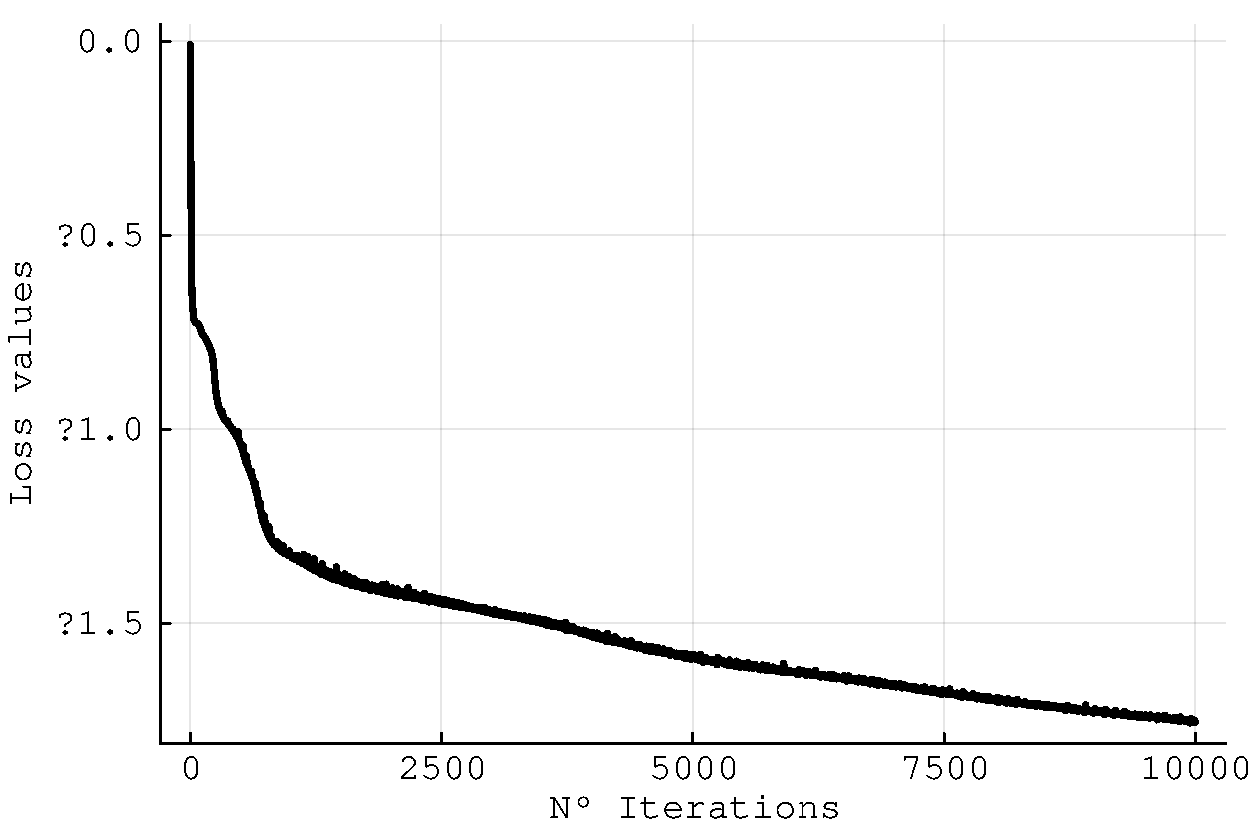
\includegraphics[width=0.45\linewidth]{Figures/NeuralNetworkStudy/Loss_corrected_V3_L4_N10_E2077_NN50.jpg}} \\
    \subfloat[Evolution of the loss function for the  architecture: 10 layers | 20 neurons | 2077 experiments | 50 nodes]{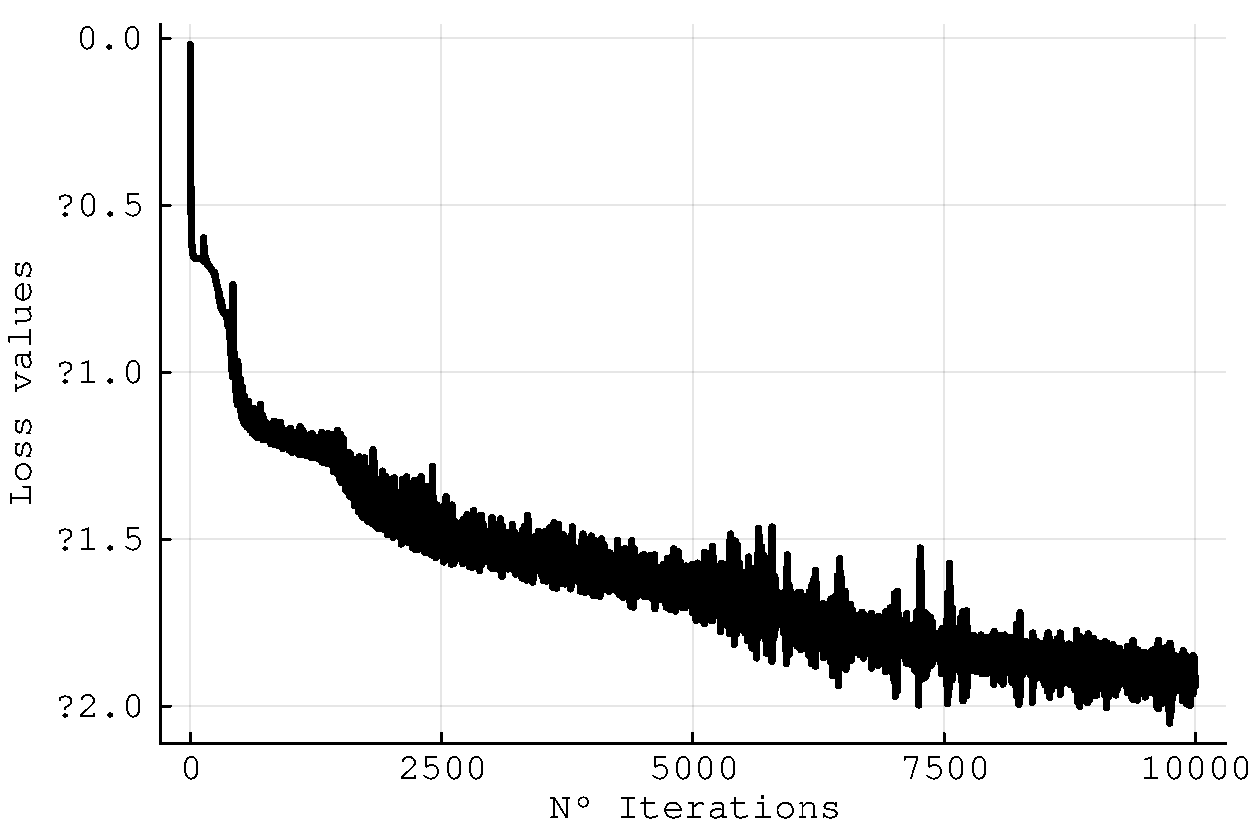
\includegraphics[width=0.45\linewidth]{Figures/NeuralNetworkStudy/Loss_corrected_V3_L10_N20_E2077_NN50.jpg}} \qquad
    \subfloat[Evolution of the loss function for the  architecture: 8 layers | 40 neurons | 2077 experiments | 200 nodes]{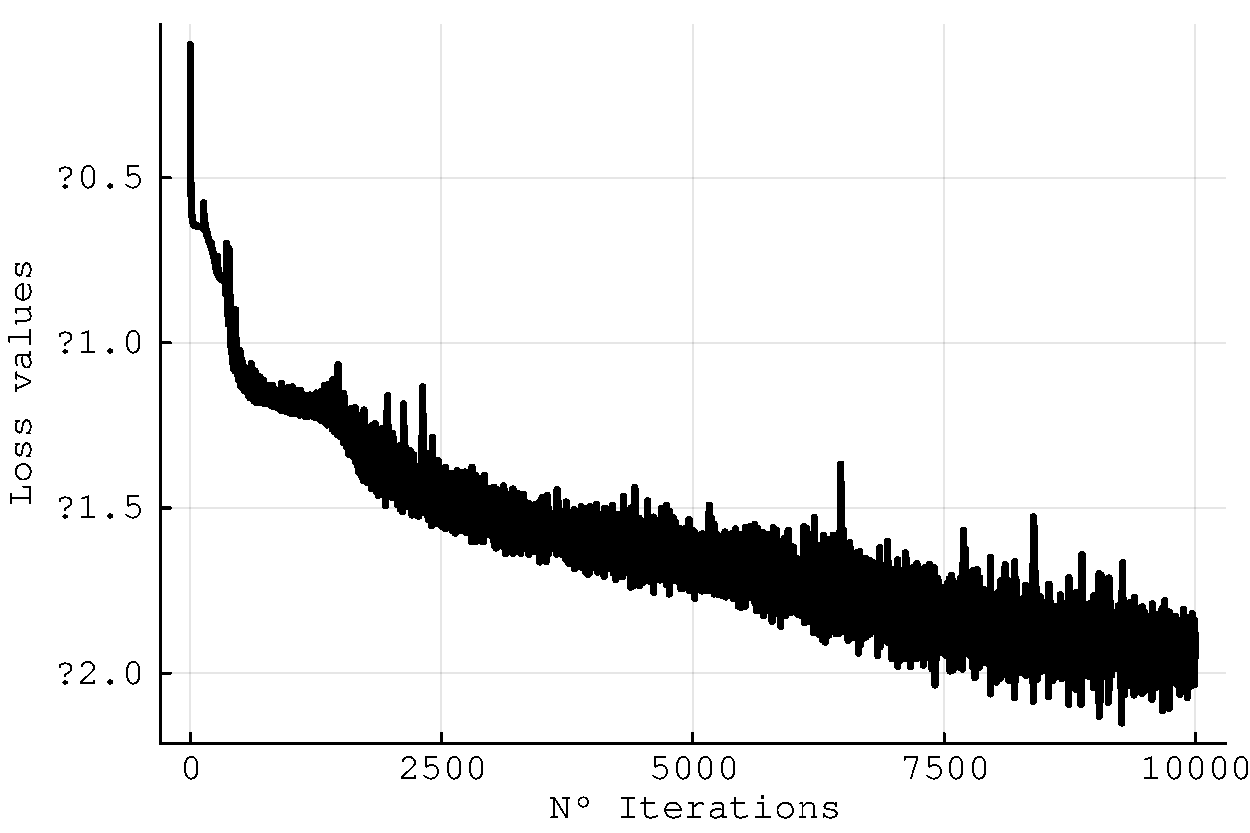
\includegraphics[width=0.45\linewidth]{Figures/NeuralNetworkStudy/Loss_corrected_V3_L8_N40_E2077_NN200.jpg}} 
  \end{center}
  \caption{Loss function during the training for the best performant neural network configuration, and 3 other architectures. Convergence is not fully achieved in every training architecture, however a high enough R2 is reached. This effectively means that further trainig the model would cause overfitting. Spikes can be seen in in the loss function during the training process, which are caused by a high value of the $\eta$ parameter in the Adam optimizer. This means that the loss is minimized quicker, at the expense of bigger fluctuating values. This strikes a good balance between effectiveness and precision.}
  \label{fig: losses}
\end{figure}
\pagebreak

Besides the R2 measurement and scatter plot of predicted displacements versus FE generated data, we tracked the trajectory of certain points in the mesh throughout the deformation of the dielectric. By applying a combination of potentials in the electrodes and measuring the elastomer's response, we can compare that displacement against the one predicted by the neural network architecture. This can provide a better outlook on how accurately the machine learning model is predicting the real response of the dielectric. 

%
% \begin{figure}[H]
%  \centering 
%   \subfloat[Trajectory tracking of point 1 in the first axis of the coordinate system]{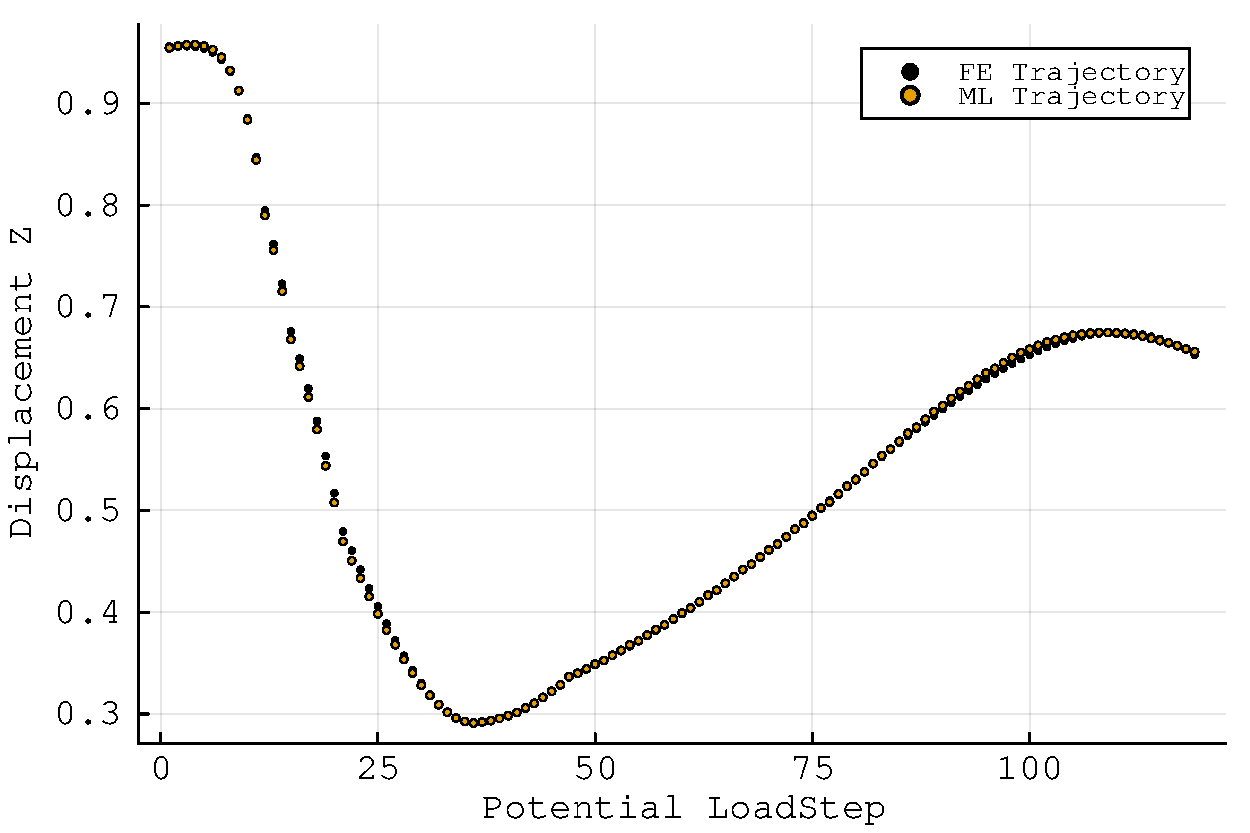
\includegraphics[width=0.45\linewidth]{Figures/NeuralNetworkStudy/Trajectory_03_009_0162_0066_P1_Coord1.jpg}}
%   \subfloat[Trajectory tracking of point 1 in the third axis of the coordinate system]{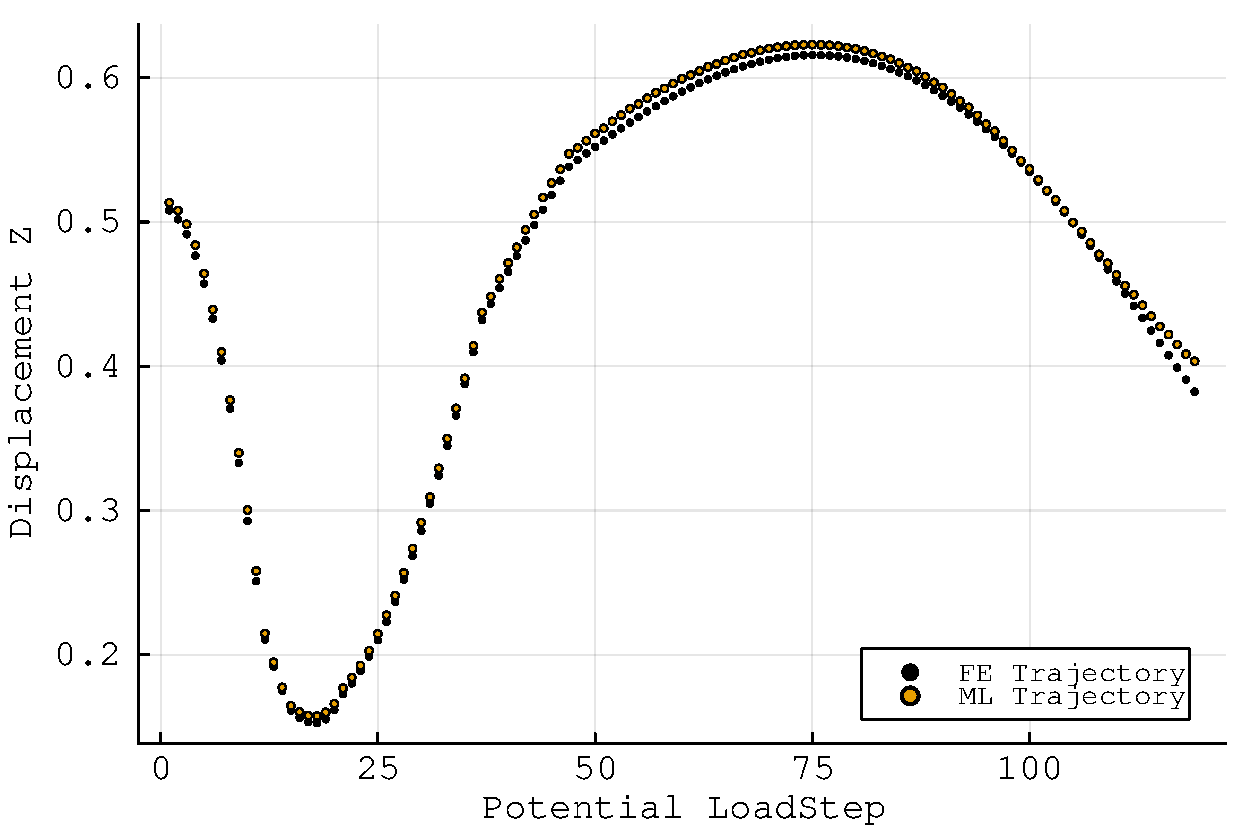
\includegraphics[width=0.45\linewidth]{Figures/NeuralNetworkStudy/Trajectory_03_009_0162_0066_P1_Coord3.jpg}}\\
%   \subfloat[Trajectory tracking of point 100 in the first axis of the coordinate system]{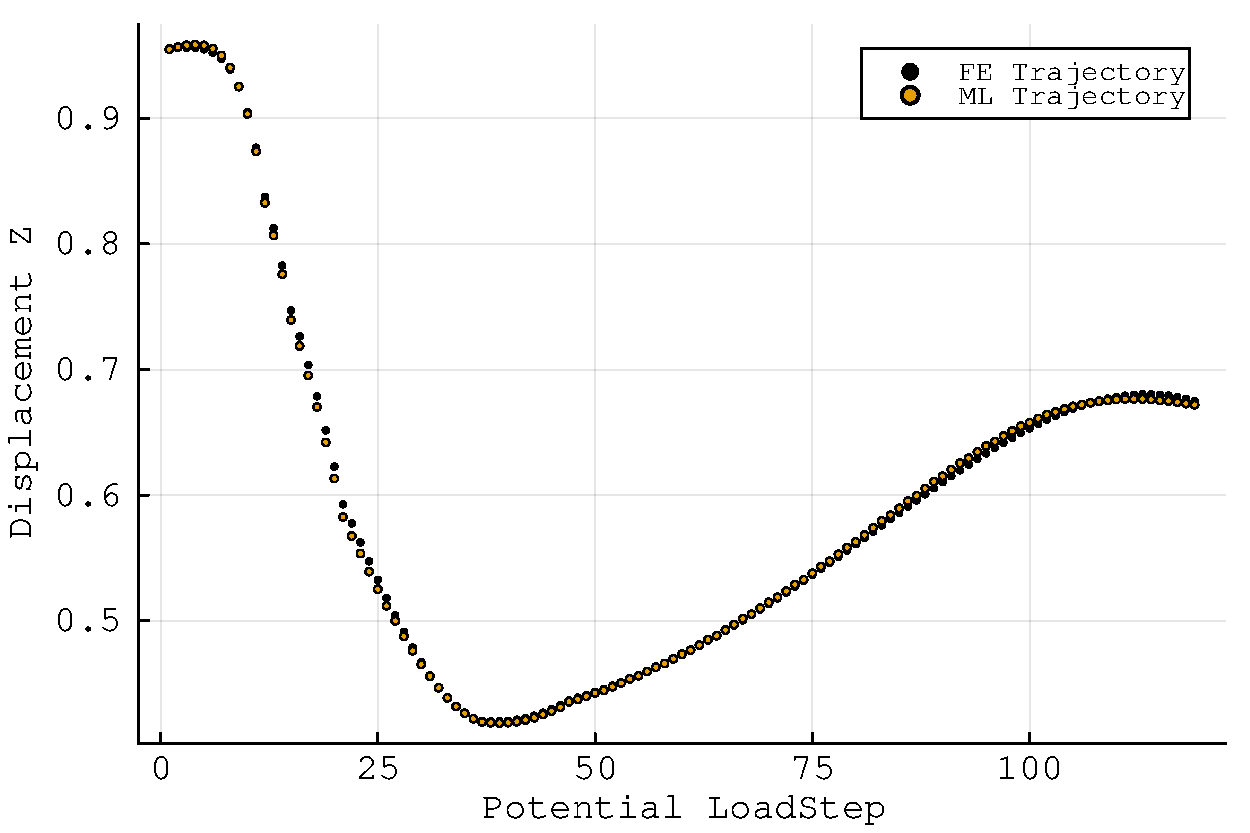
\includegraphics[width=0.45\linewidth]{Figures/NeuralNetworkStudy/Trajectory_03_009_0162_0066_P100_Coord1.jpg}}
%   \subfloat[Trajectory tracking of point 100 in the third axis of the coordinate system]{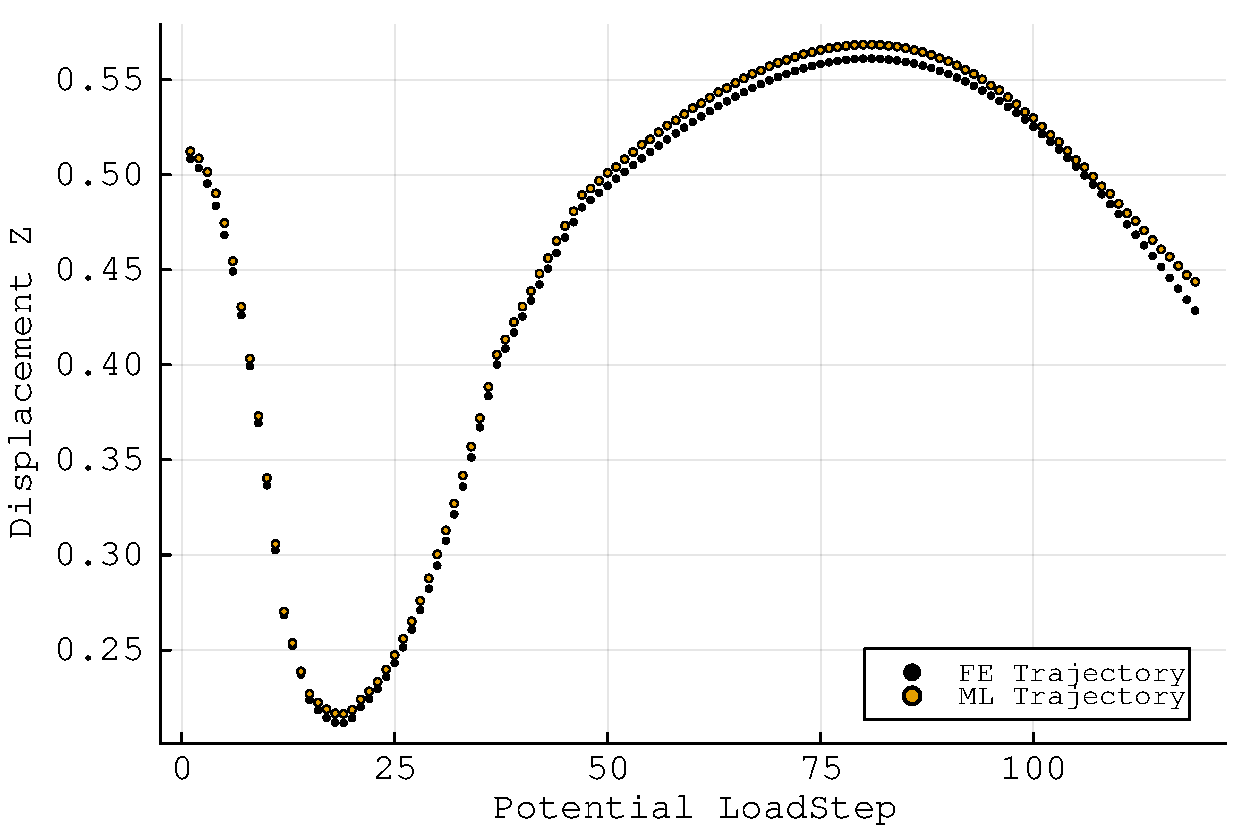
\includegraphics[width=0.45\linewidth]{Figures/NeuralNetworkStudy/Trajectory_03_009_0162_0066_P100_Coord3.jpg}}\\
%   \subfloat[Trajectory tracking of point 150 in the first axis of the coordinate system]{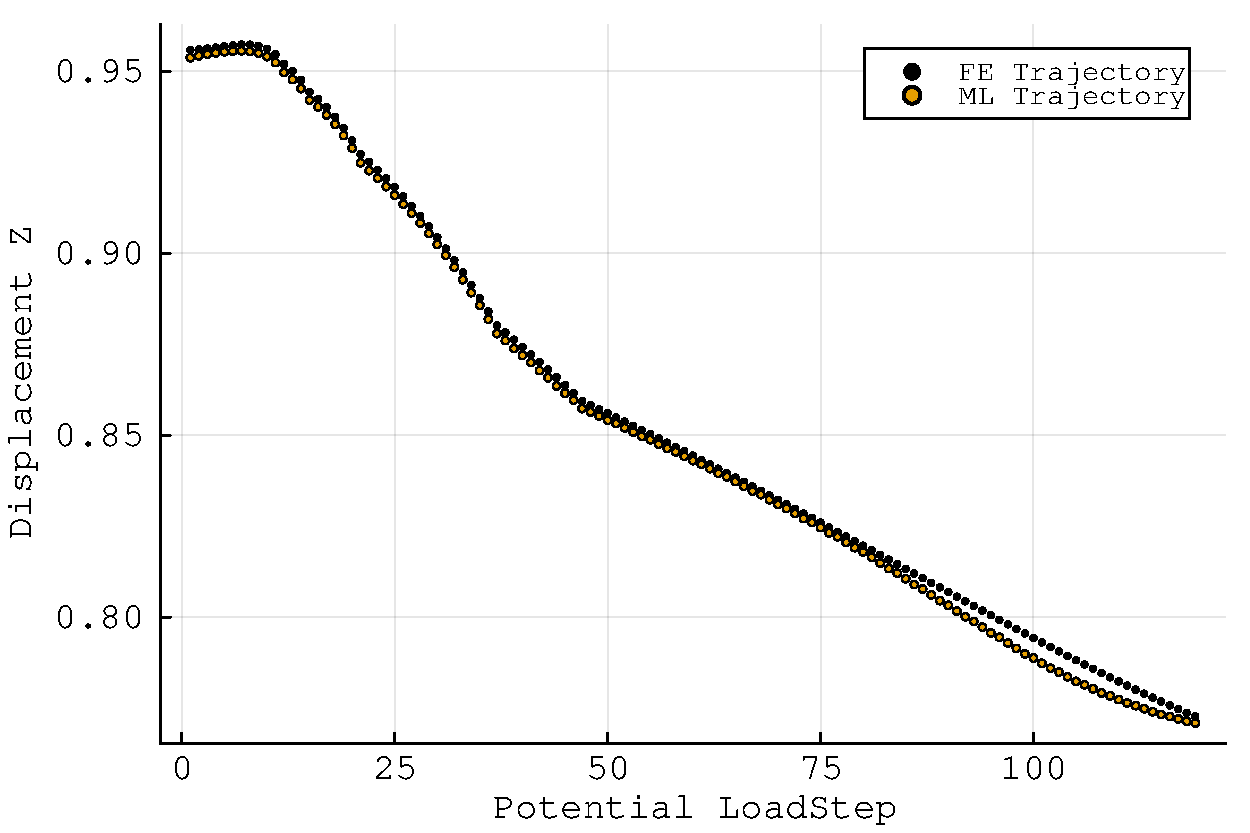
\includegraphics[width=0.45\linewidth]{Figures/NeuralNetworkStudy/Trajectory_03_009_0162_0066_P150_Coord1.jpg}}
%   \subfloat[Trajectory tracking of point 150 in the third axis of the coordinate system]{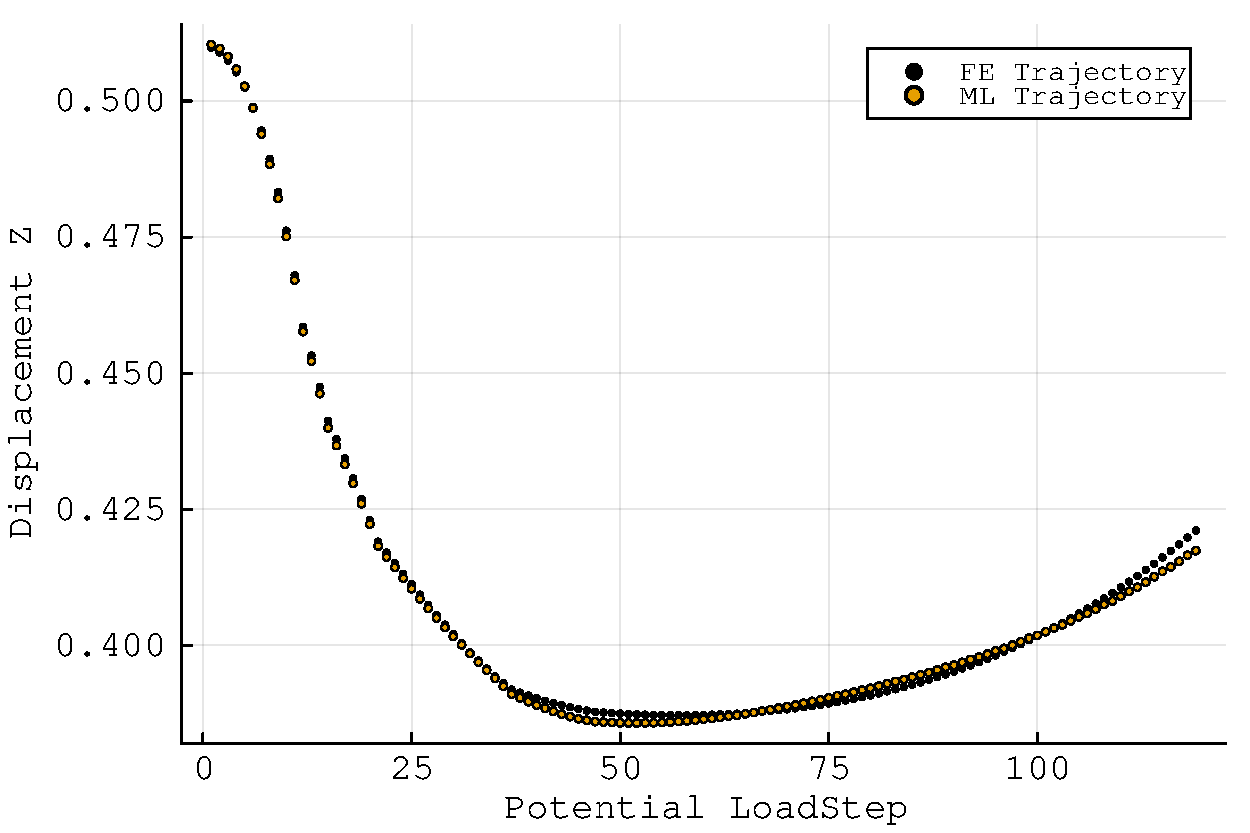
\includegraphics[width=0.45\linewidth]{Figures/NeuralNetworkStudy/Trajectory_03_009_0162_0066_P150_Coord3.jpg}}\\
% \end{figure}
% \begin{figure}[H]
%   \centering
%   \subfloat[Trajectory tracking of point 200 in the first axis of the coordinate system]{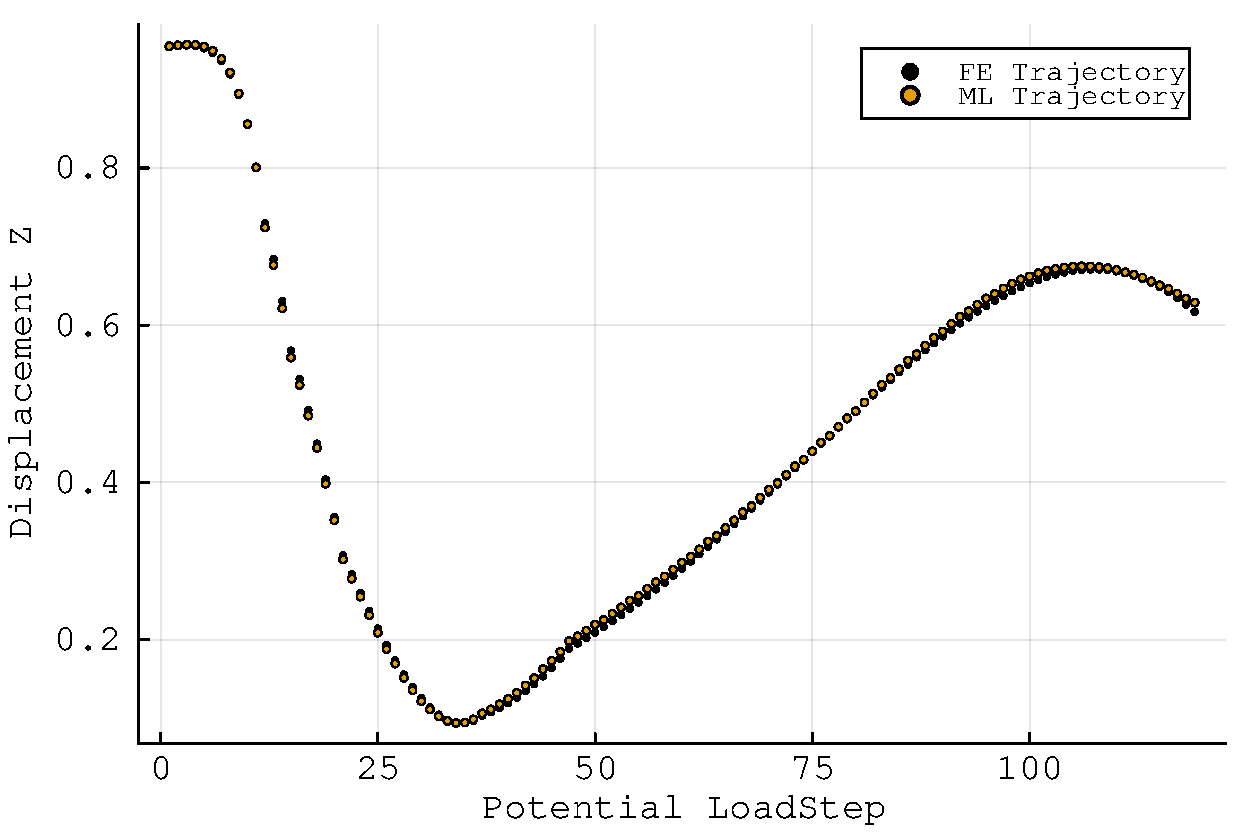
\includegraphics[width=0.45\linewidth]{Figures/NeuralNetworkStudy/Trajectory_03_009_0162_0066_P200_Coord1.jpg}}
%   \subfloat[Trajectory tracking of point 200 in the third axis of the coordinate system]{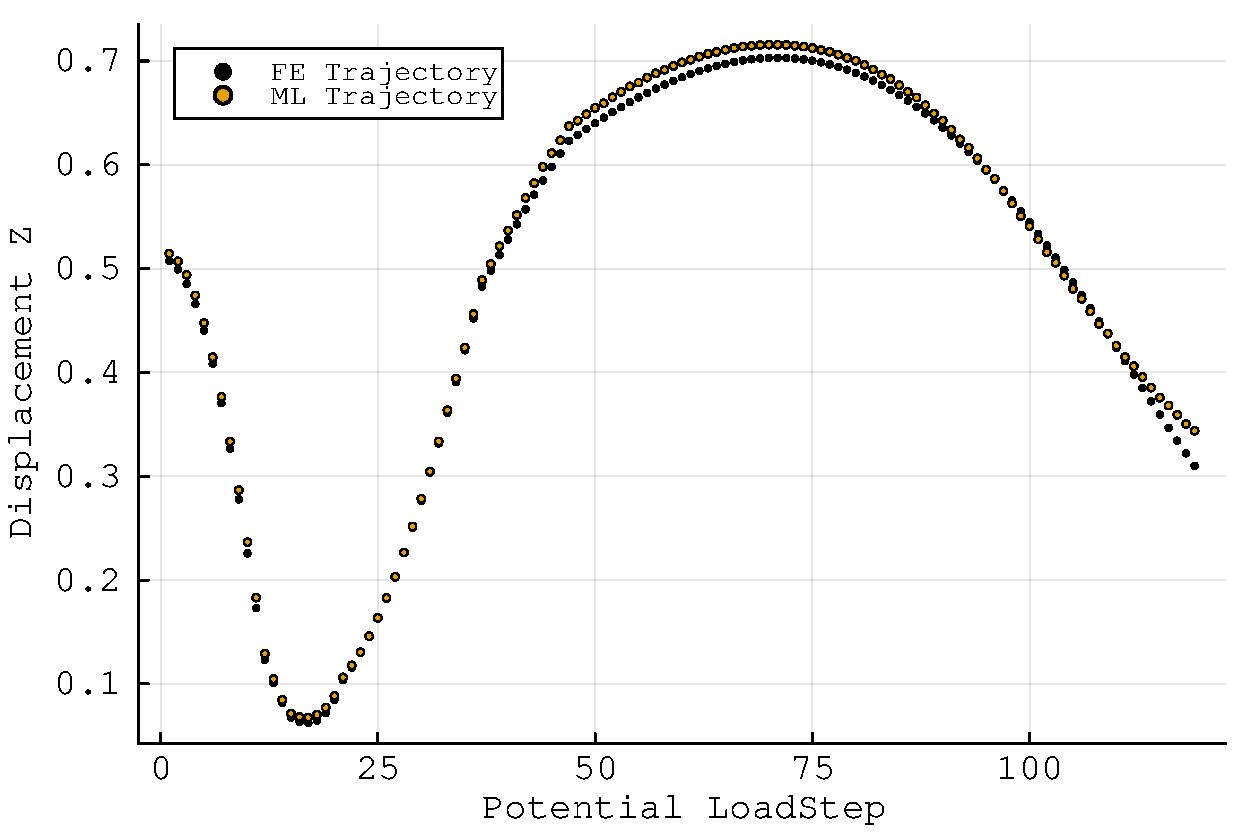
\includegraphics[width=0.45\linewidth]{Figures/NeuralNetworkStudy/Trajectory_03_009_0162_0066_P200_Coord3.jpg}}
%
%   \caption{Trajectory plot of points 1, 100, 150 and 200 for displacements in X and Z, with a potential combination in the electrodes of [0.3,0.09,.0.162,0.066] Comparison of the computed trajectory using the traditional FE implementation against the best-performing Machine Learning model. It can be seen that the trajectories are similar across different points, which is in accordance with the high R2 predicted. There is a slight discrepancy in the prediction of the displacement in Z direction, which becomes more evident towards the end of the trajectory.}
% \label{fig: Trajectories_2D}
% \end{figure} 

\begin{figure}[H]
 \centering 
  \subfloat[Trajectory of point 1 in the X axis for potential (0.006,0.03,0.27,0.3)]{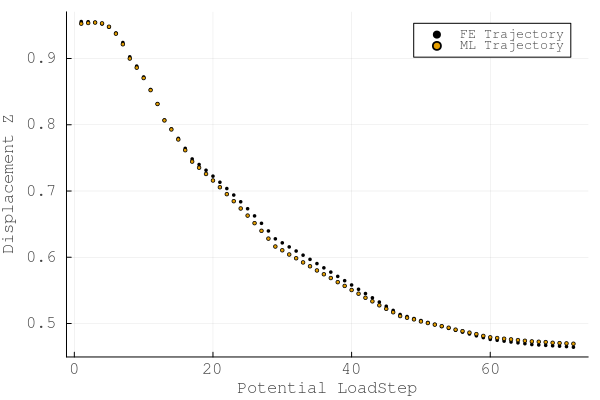
\includegraphics[width=0.45\linewidth]{Figures/NeuralNetworkStudy/Trajectory_0006_003_027_03_P1_Coord1.png}}
  \subfloat[Trajectory of point 1 in the Z axis for potential (0.006,0.03,0.27,0.3)]{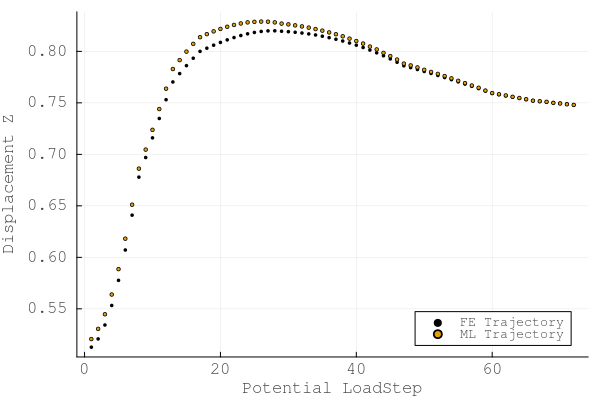
\includegraphics[width=0.45\linewidth]{Figures/NeuralNetworkStudy/Trajectory_0006_003_027_03_P1_Coord3.png}}\\
  \subfloat[Trajectory of point 1 in the X axis for potential (0.078,0.198,0.006,0.0)]{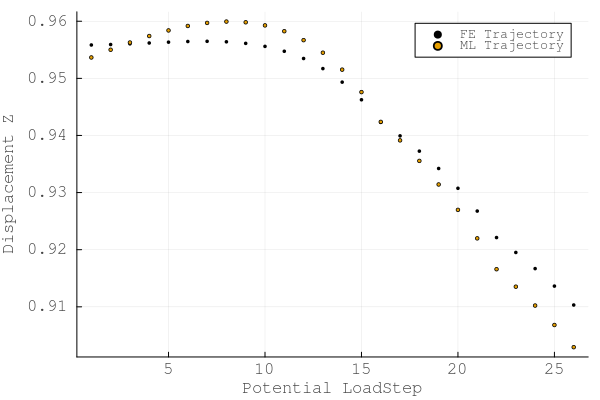
\includegraphics[width=0.45\linewidth]{Figures/NeuralNetworkStudy/Trajectory_0078_0198_0006_00_P1_Coord1.png}}
  \subfloat[Trajectory of point 1 in the Z axis for potential (0.078,0.198,0.006,0.0)]{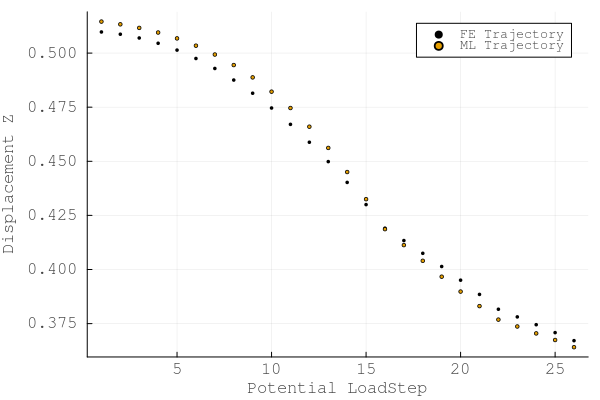
\includegraphics[width=0.45\linewidth]{Figures/NeuralNetworkStudy/Trajectory_0078_0198_0006_00_P1_Coord3.png}}\\
  \subfloat[Trajectory of point 1 in the X axis for potential (0.15,0.198,0.3,0.294)]{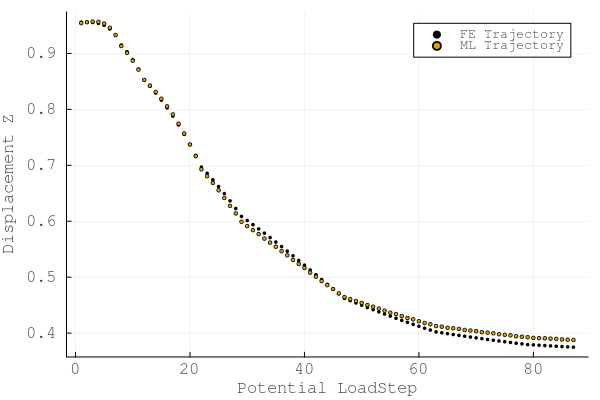
\includegraphics[width=0.45\linewidth]{Figures/NeuralNetworkStudy/Trajectory_015_0198_03_0294_P1_Coord1.png}}
  \subfloat[Trajectory of point 1 in the Z axis for potential (0.15,0.198,0.3,0.294)]{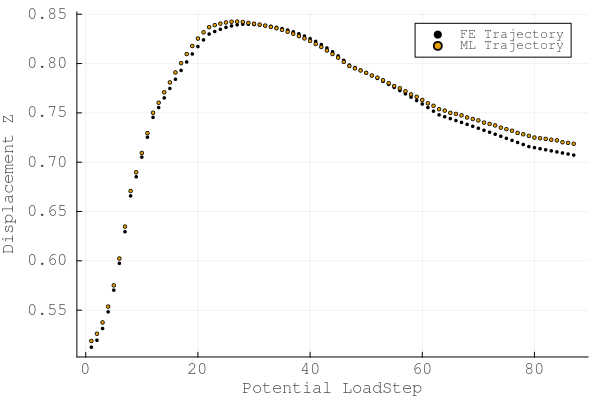
\includegraphics[width=0.45\linewidth]{Figures/NeuralNetworkStudy/Trajectory_015_0198_03_0294_P1_Coord3.png}}\\
\end{figure}
  \begin{figure}[H]
    \centering
  \subfloat[Trajectory of point 1 in the X axis for potential (0.246,0.0,0.09,0.102)]{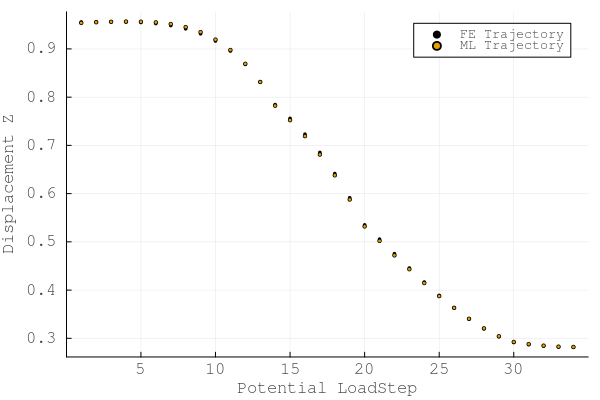
\includegraphics[width=0.45\linewidth]{Figures/NeuralNetworkStudy/Trajectory_0246_00_009_0102_P1_Coord1.png}}
  \subfloat[Trajectory of point 1 in the Z axis for potential (0.246,0.0,0.09,0.102)]{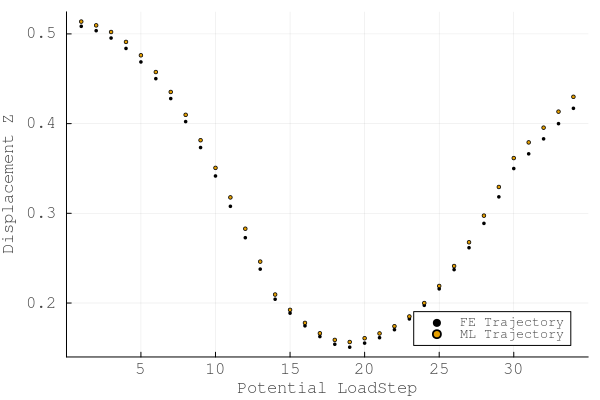
\includegraphics[width=0.45\linewidth]{Figures/NeuralNetworkStudy/Trajectory_0246_00_009_0102_P1_Coord3.png}}
  \caption{Trajectory plot of points 1 in X and Z, with multiple potential combinations in the electrodes. Comparison of the computed trajectory using the traditional FE implementation against the best-performing Machine Learning model. It can be seen that the trajectories are similar across different points, which is in accordance with the high R2 predicted.}
\label{fig: Trajectories_2D}
\end{figure}



\pagebreak
The same data can be visualized in a 3D environment, where the overall deformation of the elastomer, computed via FE, can be visualized in Paraview. The predicted displacement of a node in the mesh can be superimposed to the 3D deformation to verify that, indeed, the overall behaviour of the elastomer can be predicted using the proposed Neural Network.

\begin{figure}[H]
  \centering
  \subfloat[Frame 1]{\includegraphics[width=0.45\textwidth]{Figures/NeuralNetworkStudy/Paraview_03_009_0162_0066_FRAME1.png}}
  \subfloat[Frame 2]{\includegraphics[width=0.45\textwidth]{Figures/NeuralNetworkStudy/Paraview_03_009_0162_0066_FRAME2.png}}\\
  \subfloat[Frame 3]{\includegraphics[width=0.45\textwidth]{Figures/NeuralNetworkStudy/Paraview_03_009_0162_0066_FRAME3.png}}
  \subfloat[Frame 4]{\includegraphics[width=0.45\textwidth]{Figures/NeuralNetworkStudy/Paraview_03_009_0162_0066_FRAME4.png}}\\
\end{figure}
\begin{figure}[H]
  \centering
  \subfloat[Frame 5]{\includegraphics[width=0.45\textwidth]{Figures/NeuralNetworkStudy/Paraview_03_009_0162_0066_FRAME5.png}}
  \subfloat[Frame 6]{\includegraphics[width=0.45\textwidth]{Figures/NeuralNetworkStudy/Paraview_03_009_0162_0066_FRAME6.png}}\\
  \subfloat[Frame 7]{\includegraphics[width=0.45\textwidth]{Figures/NeuralNetworkStudy/Paraview_03_009_0162_0066_FRAME7.png}}
  \subfloat[Frame 8]{\includegraphics[width=0.45\textwidth]{Figures/NeuralNetworkStudy/Paraview_03_009_0162_0066_FRAME8.png}}
  \caption{Trajectory plot  for the potential combination of [0.3,0.09,.0.162,0.066]. The 3D data corresponds to the FE solution, and the point trajectory to the predicted displacement of point 1 using the best performing neural network architecture.}\label{fig:}
\end{figure}

\pagebreak

\begin{figure}
  \centering
  \subfloat[Frame 1]{\includegraphics[width=0.5\linewidth]{Figures/NeuralNetworkStudy/Paraview_0078_0198_0006_00_FRAME1.png}}
  \subfloat[Frame 2]{\includegraphics[width=0.5\linewidth]{Figures/NeuralNetworkStudy/Paraview_0078_0198_0006_00_FRAME2.png}}\\
  \subfloat[Frame 3]{\includegraphics[width=0.5\linewidth]{Figures/NeuralNetworkStudy/Paraview_0078_0198_0006_00_FRAME3.png}}
  \subfloat[Frame 4]{\includegraphics[width=0.5\linewidth]{Figures/NeuralNetworkStudy/Paraview_0078_0198_0006_00_FRAME4.png}}
  \caption{Trajectory plot  for the potential combination of [0.078,0.198,.0.006,0.0]. The 3D data corresponds to the FE solution, and the point trajectory to the predicted displacement of point 1 using the best performing neural network architecture.}\label{fig:}
\end{figure}

\begin{figure}
  \centering
  \subfloat[Frame 1]{\includegraphics[width=0.5\linewidth]{Figures/NeuralNetworkStudy/Paraview_0006_003_027_03_FRAME1.png}}
  \subfloat[Frame 2]{\includegraphics[width=0.5\linewidth]{Figures/NeuralNetworkStudy/Paraview_0006_003_027_03_FRAME2.png}}\\
  \subfloat[Frame 3]{\includegraphics[width=0.5\linewidth]{Figures/NeuralNetworkStudy/Paraview_0006_003_027_03_FRAME3.png}}
  \subfloat[Frame 4]{\includegraphics[width=0.5\linewidth]{Figures/NeuralNetworkStudy/Paraview_0006_003_027_03_FRAME4.png}}
  \caption{Trajectory plot  for the potential combination of [0.006,0.03,.0.27,0.3]. The 3D data corresponds to the FE solution, and the point trajectory to the predicted displacement of point 1 using the best performing neural network architecture.}\label{fig:}
\end{figure}

\begin{figure}
  \centering
  \subfloat[Frame 1]{\includegraphics[width=0.5\linewidth]{Figures/NeuralNetworkStudy/Paraview_0006_03_015_0282_FRAME1.png}}
  \subfloat[Frame 2]{\includegraphics[width=0.5\linewidth]{Figures/NeuralNetworkStudy/Paraview_0006_03_015_0282_FRAME2.png}}\\
  \subfloat[Frame 3]{\includegraphics[width=0.5\linewidth]{Figures/NeuralNetworkStudy/Paraview_0006_03_015_0282_FRAME3.png}}
  \subfloat[Frame 4]{\includegraphics[width=0.5\linewidth]{Figures/NeuralNetworkStudy/Paraview_0006_03_015_0282_FRAME4.png}}
  \caption{Trajectory plot  for the potential combination of [0.006,0.3,.0.15,0.282]. The 3D data corresponds to the FE solution, and the point trajectory to the predicted displacement of point 1 using the best performing neural network architecture.}\label{fig:}
\end{figure}

\begin{figure}
  \centering
  \subfloat[Frame 1]{\includegraphics[width=0.5\linewidth]{Figures/NeuralNetworkStudy/Paraview_0078_03_0138_0006_FRAME1.png}}
  \subfloat[Frame 2]{\includegraphics[width=0.5\linewidth]{Figures/NeuralNetworkStudy/Paraview_0078_03_0138_0006_FRAME2.png}}\\
  \subfloat[Frame 3]{\includegraphics[width=0.5\linewidth]{Figures/NeuralNetworkStudy/Paraview_0078_03_0138_0006_FRAME3.png}}
  \subfloat[Frame 4]{\includegraphics[width=0.5\linewidth]{Figures/NeuralNetworkStudy/Paraview_0078_03_0138_0006_FRAME4.png}}
  \caption{Trajectory plot  for the potential combination of [0.078,0.3,.0.138,0.006]. The 3D data corresponds to the FE solution, and the point trajectory to the predicted displacement of point 1 using the best performing neural network architecture.}\label{fig:}
\end{figure}

\begin{figure}
  \centering
  \subfloat[Frame 1]{\includegraphics[width=0.5\linewidth]{Figures/NeuralNetworkStudy/Paraview_027_00_015_0162_FRAME1.png}}
  \subfloat[Frame 2]{\includegraphics[width=0.5\linewidth]{Figures/NeuralNetworkStudy/Paraview_027_00_015_0162_FRAME2.png}}\\
  \subfloat[Frame 3]{\includegraphics[width=0.5\linewidth]{Figures/NeuralNetworkStudy/Paraview_027_00_015_0162_FRAME3.png}}
  \subfloat[Frame 4]{\includegraphics[width=0.5\linewidth]{Figures/NeuralNetworkStudy/Paraview_027_00_015_0162_FRAME4.png}}
  \caption{Trajectory plot  for the potential combination of [0.27,0.0,.0.15,0.162]. The 3D data corresponds to the FE solution, and the point trajectory to the predicted displacement of point 1 using the best performing neural network architecture.}\label{fig:}
\end{figure}


\subsection{Second example: 20-electrode dielectric elastomer}

\subsubsection{Data generation}

The second example consists of a 20-electrode dielectric elastomer, whose electrodes are positioned in the top and middle surfaces. This configuration allows for more exotic deformation responses of the dielectric elastomers, including torsion, bending and a combination of both movements.


\subsubsection{Training strategy}
\subsubsection{Results}

For each of the hyperparameters specified, the values studied were the following:

\begin{table}[!hb]
  \centering
\begin{tabular}{l|cccc}
\textbf{Parameters} & \multicolumn{3}{c}{\textbf{Value}} \\ \hline
Layers              & 4      & 8       & 10            \\
Neurons             & 10     & 20      & 40           \\
Experiments         & 2077    & 7000    & 10000      \\
Nodes               & 50     & 10      & 200           \\
Epochs              &  \multicolumn{3}{c}{1e4}        
\end{tabular}
  \caption{Values used in the parametric study during the training phase. Every combination of these parameters was analysed and parsed to obtain the best performing architecture.}
\end{table}







\begin{table}[!hb]
\centering
\begin{minipage}{.45\textwidth}

\begin{tabular}{lllllllcc|ccc}
\multicolumn{9}{c|}{\multirow{2}{*}{\begin{tabular}[c]{@{}c@{}}$n_{nodes}=50$\\ $n_{experiments}=2077$\end{tabular}}} & \multicolumn{3}{c}{$n_{neurons}$} \\
\multicolumn{9}{c|}{}                                                                                                 & 10        & 20        & 40        \\ \hline
        &         &         &         &         &         &         & \multirow{4}{*}{\rotatebox{90}{$n_{layers}$}}        & 4        &  0.9969        &  0.9971        &  0.9990        \\
        &         &         &         &         &         &         &                                      & 8        &  0.9960        &  0.9985       &  0.9973        \\
        &         &         &         &         &         &         &                                      & 10        &  0.9970        &  0.9985        &  0.9990        
\end{tabular}

\end{minipage}

  \vspace{1cm}
\begin{minipage}{.45\textwidth}

\begin{tabular}{lllllllcc|ccc}
\multicolumn{9}{c|}{\multirow{2}{*}{\begin{tabular}[c]{@{}c@{}}$n_{nodes}=50$\\ $n_{experiments}=10000$\end{tabular}}} & \multicolumn{3}{c}{$n_{neurons}$} \\
\multicolumn{9}{c|}{}                                                                                                 & 10        & 20        & 40        \\ \hline
        &         &         &         &         &         &         & \multirow{4}{*}{\rotatebox{90}{$n_{layers}$}}        & 4        &  0.9953        &  0.9986        &  0.9989        \\
        &         &         &         &         &         &         &                                      & 8        &  0.9968        &  0.9982       &  0.9987        \\
        &         &         &         &         &         &         &                                      & 10        &  0.9965        &  0.9983        &  0.9990        
\end{tabular}

\end{minipage}

  \vspace{1cm}
\begin{minipage}{.45\textwidth}

\begin{tabular}{lllllllcc|ccc}
\multicolumn{9}{c|}{\multirow{2}{*}{\begin{tabular}[c]{@{}c@{}}$n_{nodes}=200$\\ $n_{experiments}=2077$\end{tabular}}} & \multicolumn{3}{c}{$n_{neurons}$} \\
\multicolumn{9}{c|}{}                                                                                                 & 10        & 20        & 40        \\ \hline
        &         &         &         &         &         &         & \multirow{4}{*}{\rotatebox{90}{$n_{layers}$}}        & 4        &  0.9966        &  0.9980        &  0.9988        \\
        &         &         &         &         &         &         &                                      & 8        &  0.9962        &  0.9982       &  0.9984        \\
        &         &         &         &         &         &         &                                      & 10        &  0.9891        &  0.9978        &  0.9977        
\end{tabular}

\end{minipage}

  \vspace{1cm}
\begin{minipage}{.45\textwidth}

\begin{tabular}{lllllllcc|ccc}
\multicolumn{9}{c|}{\multirow{2}{*}{\begin{tabular}[c]{@{}c@{}}$n_{nodes}=200$\\ $n_{experiments}=10000$\end{tabular}}} & \multicolumn{3}{c}{$n_{neurons}$} \\
\multicolumn{9}{c|}{}                                                                                                 & 10        & 20        & 40        \\ \hline
        &         &         &         &         &         &         & \multirow{4}{*}{\rotatebox{90}{$n_{layers}$}}        & 4        &  0.9944        &  0.9981        &  0.9991        \\
        &         &         &         &         &         &         &                                      & 8        &  0.9958        &  0.9976       &  0.9995        \\
        &         &         &         &         &         &         &                                      & 10        &  0.9971        &  0.9977        &  0.9969        
\end{tabular}

\end{minipage}





  \caption{R2 measurement for every combination of neurons and layers for 50 and 200 nodes and 2077 and 10000 experiments.}
  \label{tab: R2_values}
\end{table}



